\chapter{Modellazione dei Casi d'Uso}
\section{Attori e Casi d'Uso}
\begin{table}[!hbp]
	\centering
	\begin{tblr}{colspec=XX}
		\begin{minipage}[t]{\linewidth}
			\paragraph{Attori primari}
			\begin{itemize}[leftmargin=*]
				\item UtenteNonRegistrato
				\item UtenteRegistrato
				\item Utente
				\item Amministratore
			\end{itemize}
		\end{minipage} &
		\begin{minipage}[t]{\linewidth}
			\paragraph{Attori secondari}
			\begin{itemize}[leftmargin=*]
				\item SistemaGestioneAcquisti
			\end{itemize}
		\end{minipage} \\
	\end{tblr}
\end{table}
\begin{table}[!hbp]
	\centering
	\begin{tblr}{colspec=XX}
		\begin{minipage}[t]{\linewidth}
			\paragraph{Casi d'uso}
			\begin{enumerate}[leftmargin=*]
				\item Registrazione 
				\item Autenticazione
				\item RicercaEvento
				\item PubblicaEvento
				\item ConsultaEventiPubblicati
				\item PartecipazioneEvento
				\item AcquistoBiglietto
				\item ModificaDatiPersonali
				\item VisualizzaBiglietto
				\item ScaricaBiglietto
			\end{enumerate}
		\end{minipage} &
		\begin{minipage}[t]{\linewidth}
			\paragraph{Casi d'uso di inclusione}
			\begin{enumerate}[leftmargin=*]
                \item ConsultaCatalogoEventi
	      \item ConsultaStoricoBiglietti
			\end{enumerate}

		\end{minipage}
	\end{tblr}
\end{table}
\begin{table}[!ht]
\centering
\small
\begin{tblr}{
  colspec = {X[2,l] X[1.2,l] X[1.7,l] X[1.6,l] X[1.5,l]},
  hlines,
  row{1} = {font=\bfseries}
}
Caso d'uso & Attori Primari & Attori Secondari & Incl. / Ext. & Requisiti corrispondenti \\
Registrazione & UtenteNonRegistrato & -- & -- & \Req{rf}{01} \\
Autenticazione & UtenteRegistrato & -- & -- & \Req{rf}{02} \\
RicercaEvento & UtenteRegistrato & -- & -- &\Req{rf}{08} \\
PubblicaEvento & Amministratore & -- & -- & \Req{rf}{06} \\
ConsultaEventiPubblicati & Amministratore & -- & Include: Consulta Catalogo Eventi & \Req{rf}{19}, \Req{rf}{20}, \Req{rf}{21} \\
PartecipazioneEvento& Utente & -- & -- & \Req{rf}{12} \\
AcquistaBiglietto & Utente & SistemaGestioneAcquisti & Include: ConsultaCatalogoEventi & \Req{rf}{09} \\
ModificaDatiPersonali & Utente & -- & -- & \Req{rf}{05} \\
VisualizzaBiglietto & Utente & -- & -- & \Req{rf}{10} \\
ScaricaBiglietto & Utente & -- & -- & \Req{rf}{11} \\
ConsultaStoricoBiglietti & Utente & -- & --  & \Req{rf}{04} \\
ConsultaCatalogoEventi & UtenteRegistrato & --  & -- & \Req{rf}{07} \\

\end{tblr}
\end{table}

\section{Diagramma dei Casi d'Uso}
\begin{center}
\centering
	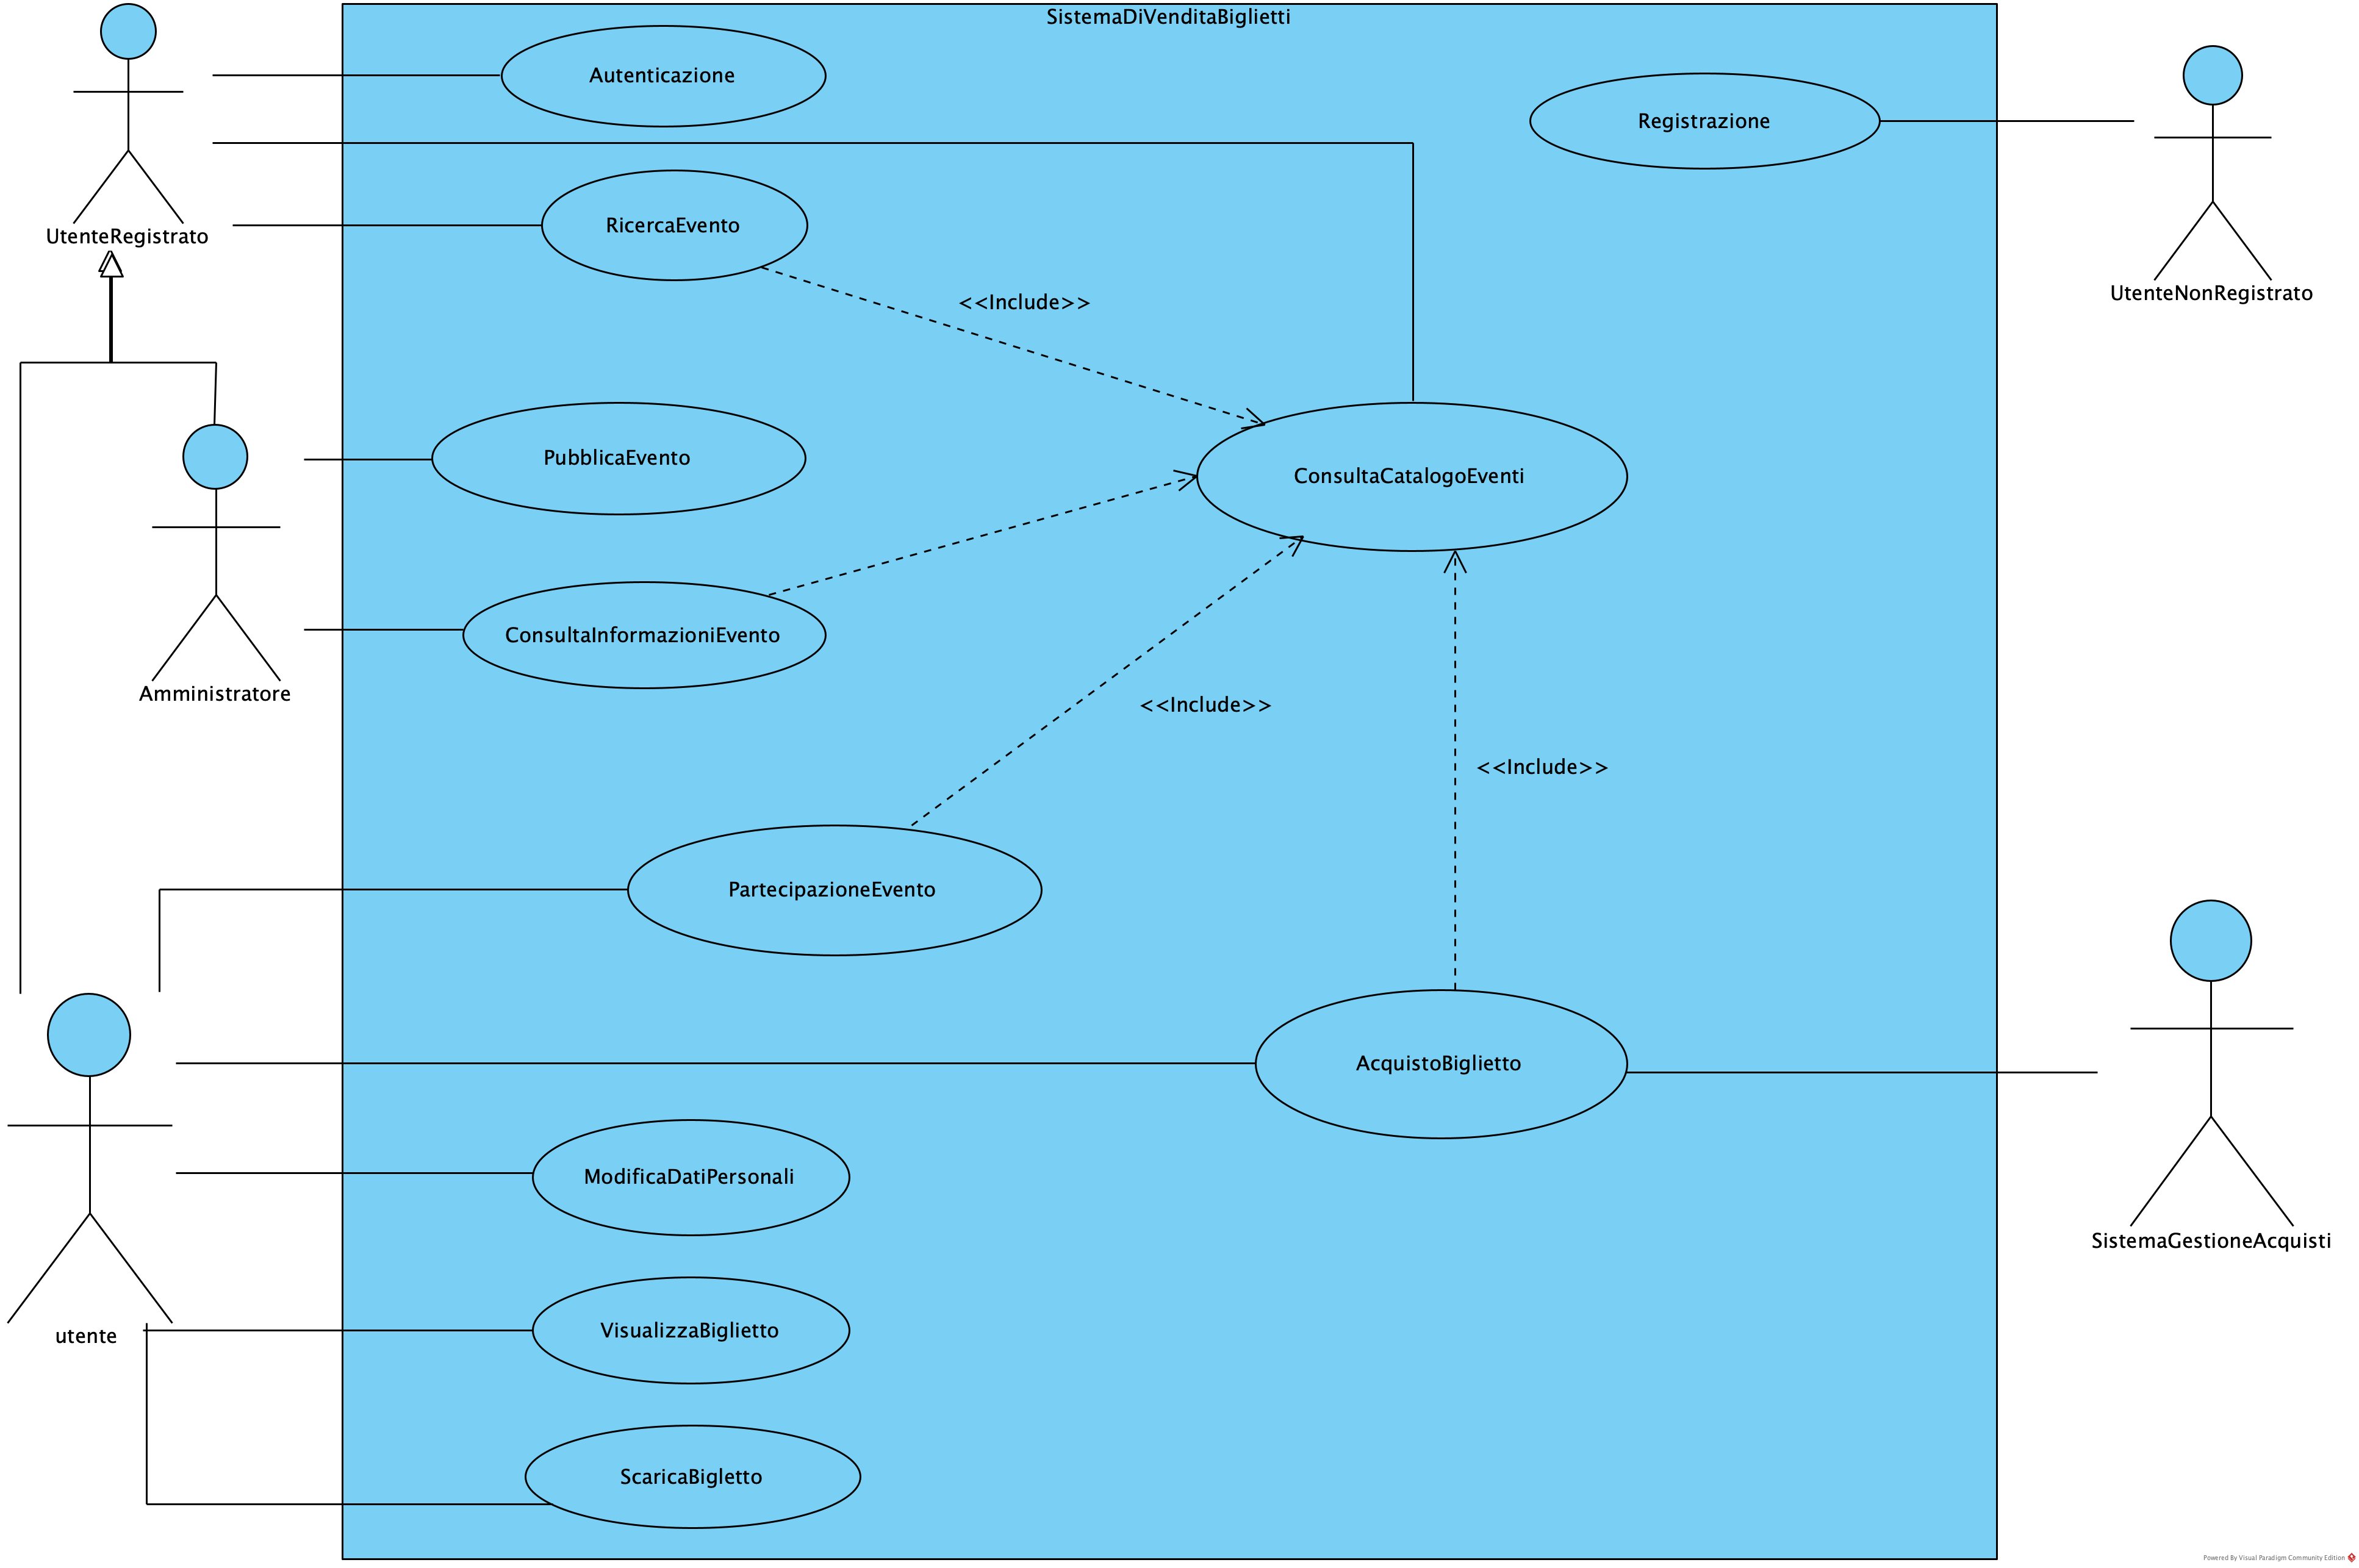
\includegraphics[width=\linewidth]{assets/casid'uso/usd.png}
\end{center}	

\clearpage
\section{Scenari}
\IncludeTable{capitoli/scenari/Registrazione}
\IncludeTable{capitoli/scenari/Autenticazione}
\IncludeTable{capitoli/scenari/ModificaDatiPersonali}
\IncludeTable{capitoli/scenari/RichiediCatalogoEventi}
\IncludeTable{capitoli/scenari/RicercaEvento}
\IncludeTable{capitoli/scenari/VisualizzaBiglietto}
\IncludeTable{capitoli/scenari/ConsultaStoricoBiglietti}
\IncludeTable{capitoli/scenari/ScaricaBiglietto}
\IncludeTable{capitoli/scenari/AcquistaBiglietto}
\IncludeTable{capitoli/scenari/PubblicaEvento}
\IncludeTable{capitoli/scenari/PartecipazioneEvento}
\IncludeTable{capitoli/scenari/ConsultaInformazioniEvento}
\clearpage
\section{Diagramma delle Classi}
Di seguito riportiamo il diagramma delle classi di analisi.
\begin{figure}[!ht]
	\centering
	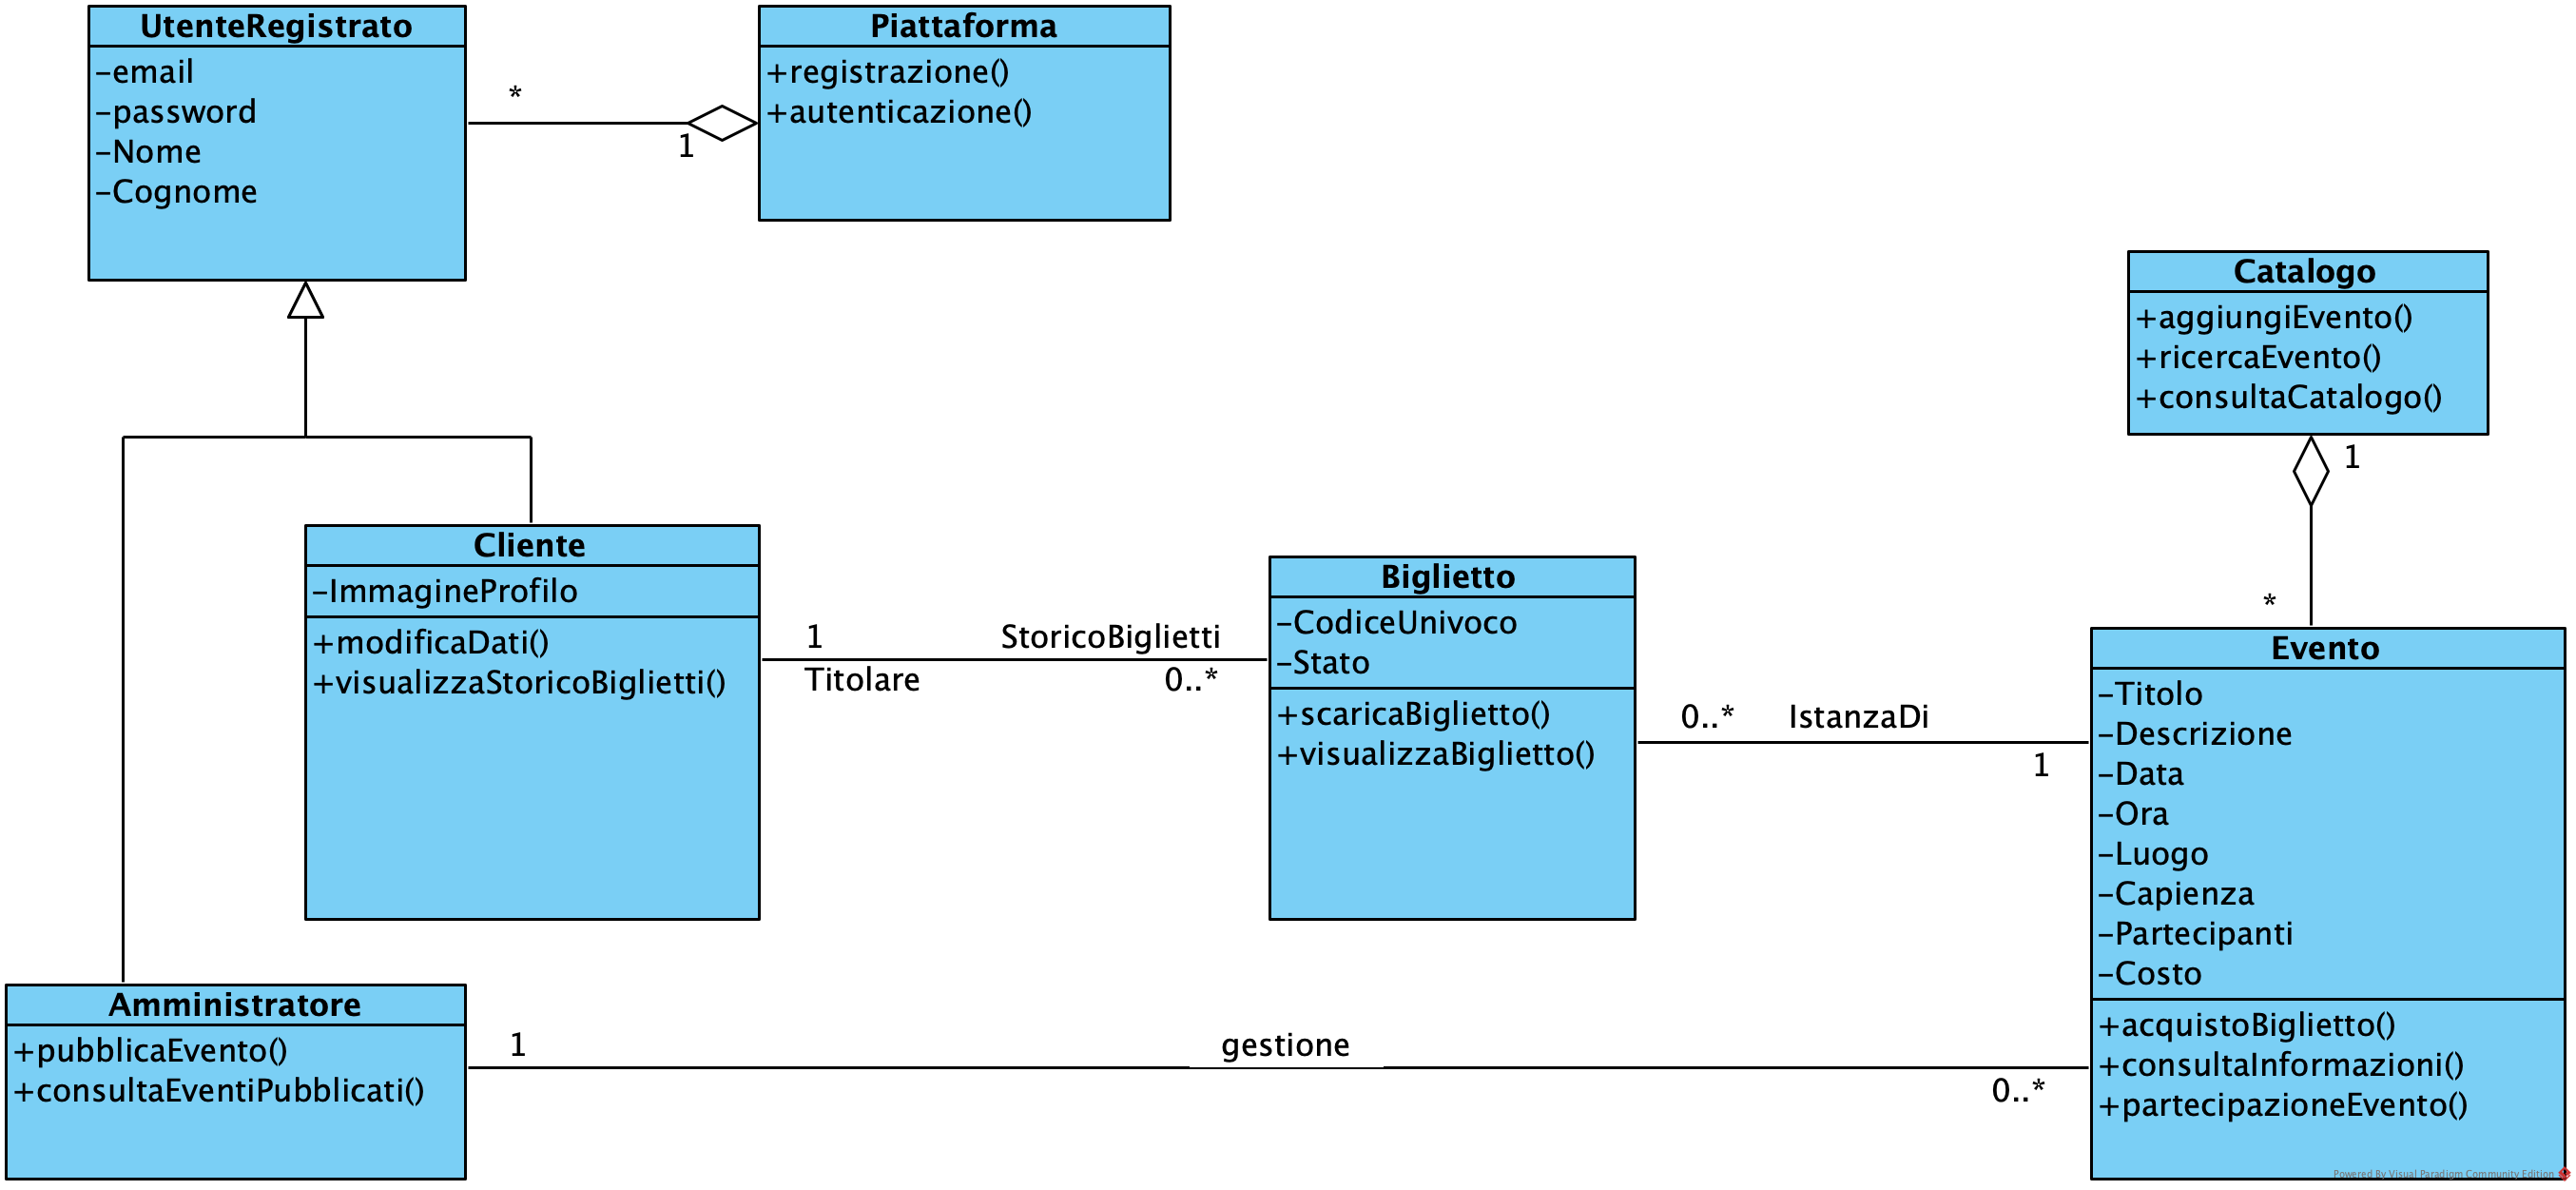
\includegraphics[width=0.8\linewidth]{assets/casid'uso/DiagrammaDelleClassi.png}
	\caption{Diagramma delle classi di analisi}
\end{figure}


\begin{table}[h]
	\centering
	\begin{tblr}{
	  colspec = {X[0.6,c] X[0.6,c]},
	  width = 1\linewidth, 
	  hlines, vlines,
	  row{1} = {bg=gray!30, font=\bfseries}
	}
	RESPONSABILITÀ & CLASSE \\
	Registrazione & SistemaGestioneEventi \\
	Autenticazione & SistemaGestioneEventi \\
	ModificaDati & Cliente \\
	VisualizzaStoricoBiglietti & Cliente \\
	CreazioneEvento & Amministratore \\
	ScaricaBiglietto & Biglietto \\
	VisualizzaBiglietto & Biglietto \\
	AcquistoBiglietto & Evento \\
	PartecipazioneEvento & Evento \\
	ConsultaInformazioni & Evento \\
	AggiungiEvento & Catalogo \\
	RicercaEvento & Catalogo \\

	\end{tblr}
\end{table}

\begin{description}
	\item Registrazione e autenticazione sono responsabilità di \textbf{SistemaGestioneEventi} in quanto \textless\textless information expert \textgreater\textgreater{} di \textit{UtenteRegistrato}.
	
	\item ModificaDati e VisualizzaStoricoBiglietti sono responsabilità di \textbf{Cliente} in quanto agiscono su suoi attributi e classi ad esso associate.
	
	\item AcquistoBiglietto è una responsabilità di \textbf{Evento} in quanto \textless\textless creator \textgreater\textgreater{} di biglietti.
	
	\item PartecipazioneEvento è una responsabilità di \textbf{Evento} seguendo il pattern \textless\textless LOW COUPLING \textgreater\textgreater.
	
	\item AggiungiEvento è una responsabilità di \textbf{Catalogo} poiché, dopo la creazione, l’evento verrà aggiunto al catalogo.
	
	\item RicercaEvento è una responsabilità di \textbf{Catalogo} essendo il contenitore degli eventi.
	
	\item CreazioneEvento è una responsabilità di \textbf{Amministratore} essendo il \textless\textless creator \textgreater\textgreater{} di Eventi.
  \end{description}


\clearpage


\section{Diagrammi di sequenza}


\subsection{Registrazione}

\begin{center}
    La creazione del seguente diagramma di sequenza, sviluppato a partire dalla descrizione dello scenario del caso d’uso \textit{Registrazione}, ha fatto emergere la necessità di definire un metodo privato specifico della classe \textbf{SistemaGestioneEventi}:

    \vspace{1ex}
    \textbf{controlloEmail(Email)}

    \vspace{2ex}
    Tale metodo consente a \textbf{SistemaGestioneEventi} di verificare che l’indirizzo email  non sia già utilizzato da un altro utente.

    \vspace{3ex}
    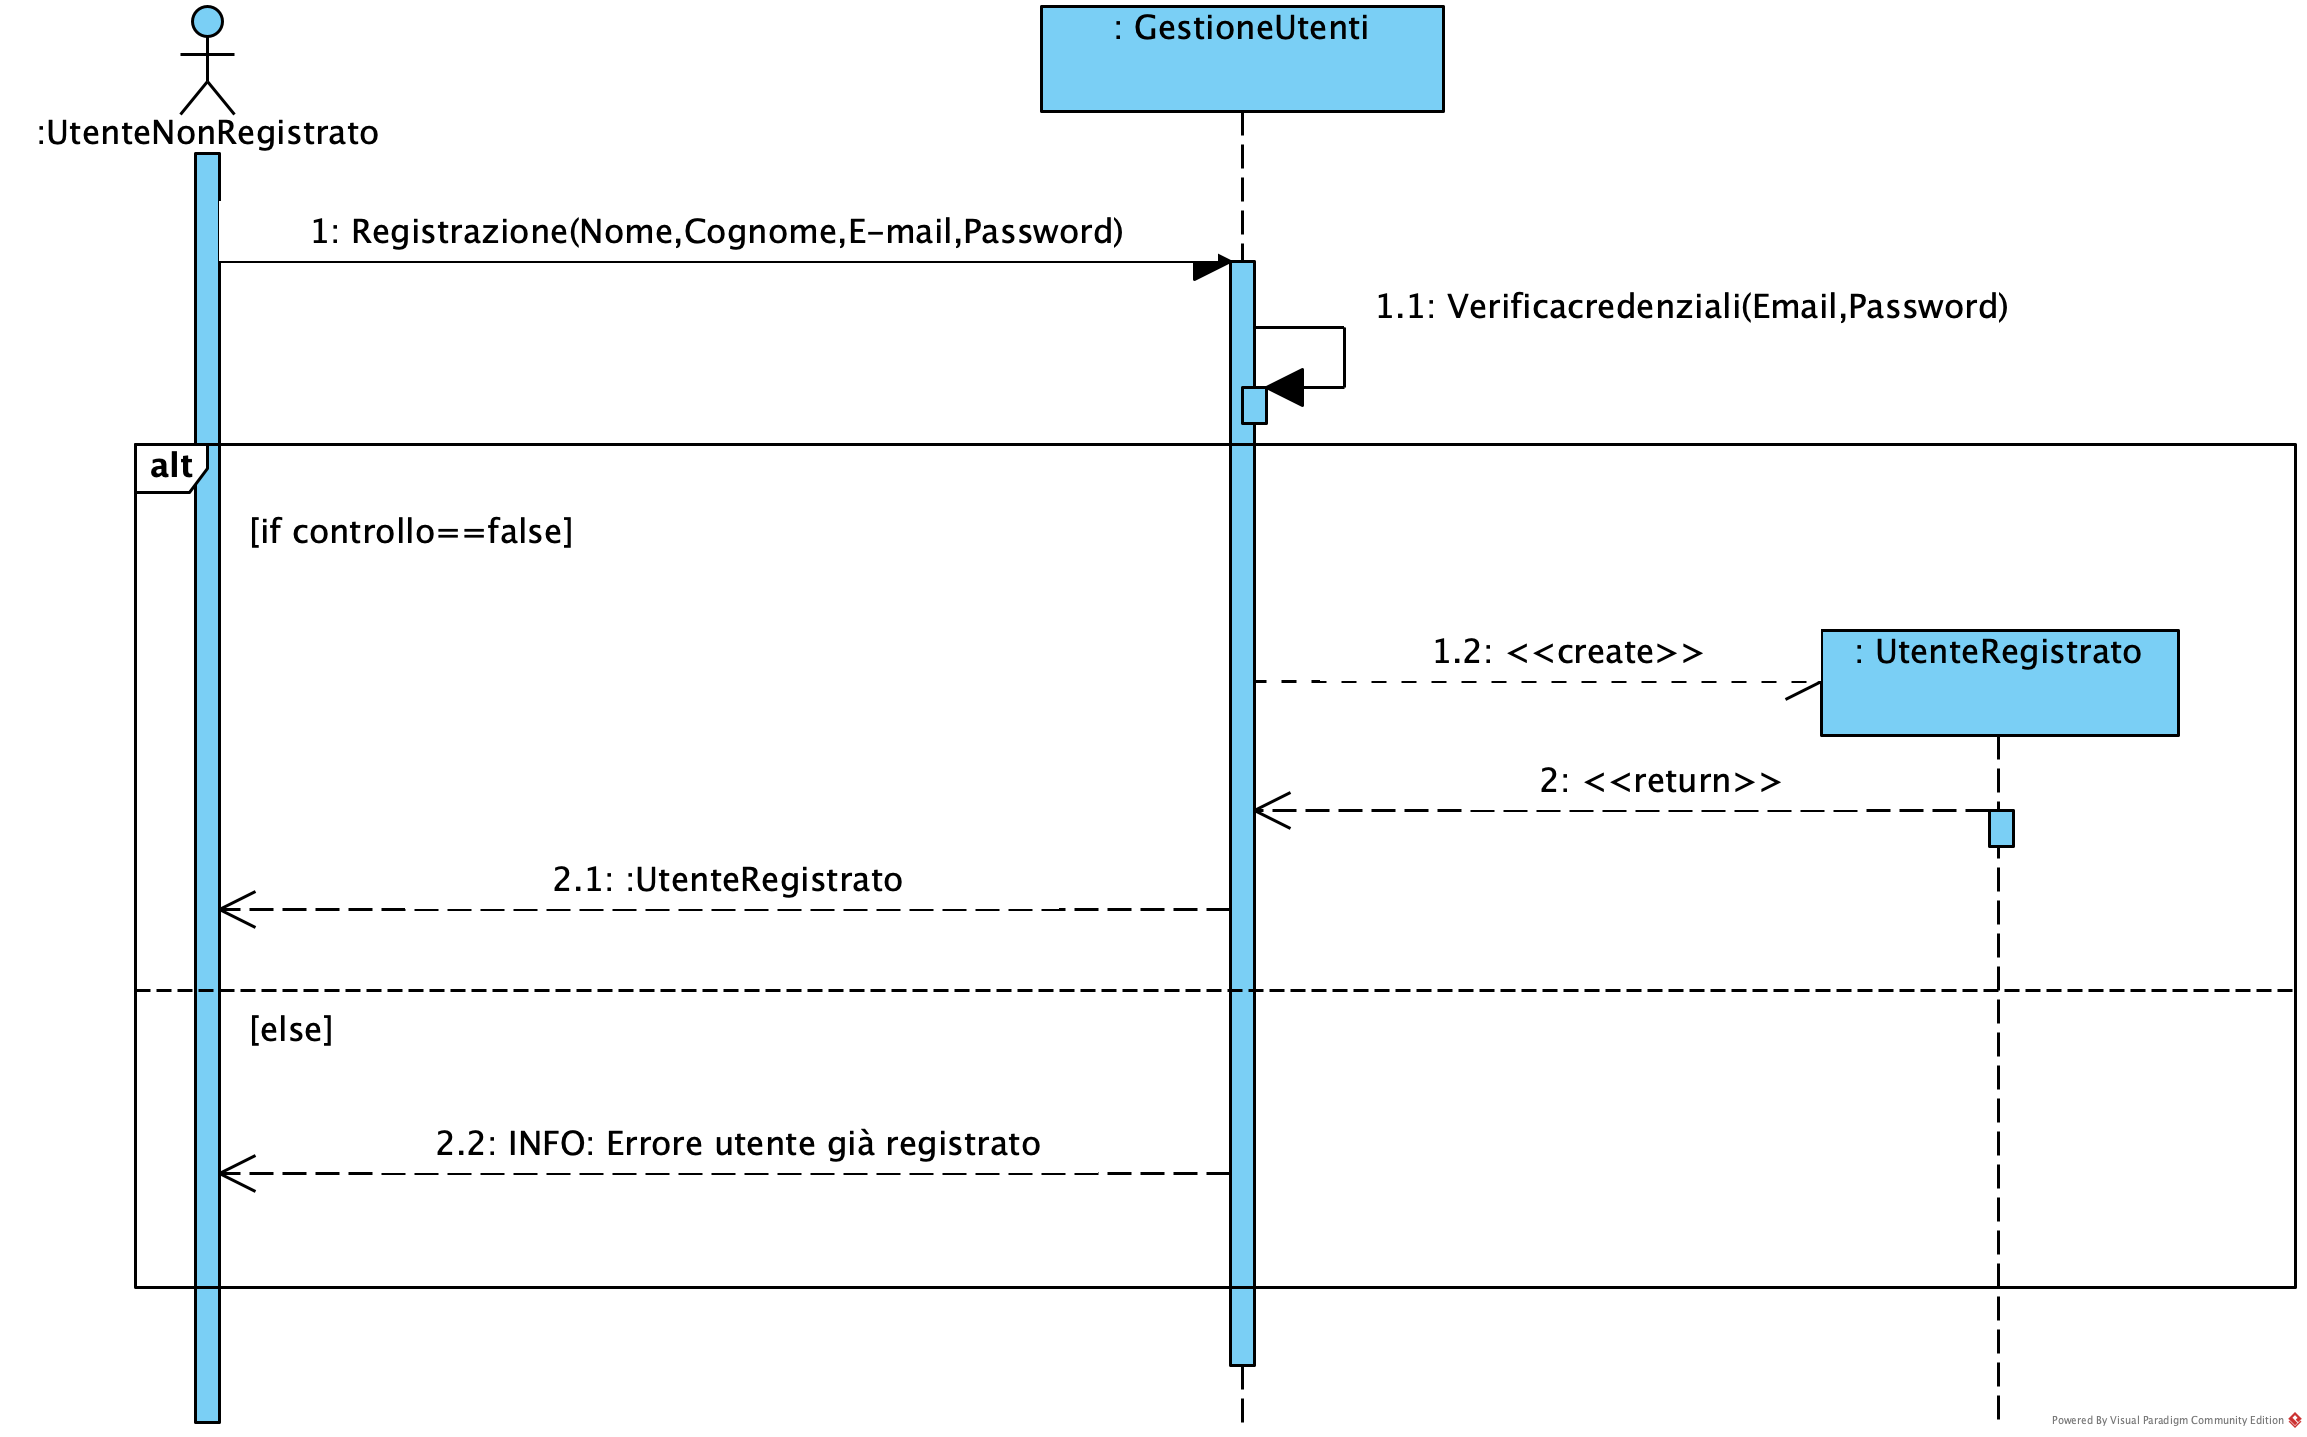
\includegraphics[width=0.8\linewidth]{assets/casid'uso/Registrazione.png}
    
    \vspace{1ex}
    \textbf{Figura:} Diagramma di sequenza per il caso d’uso \textit{Registrazione}
\end{center}

\subsection{Autenticazione}
\begin{figure}[!ht]
    \hspace*{4cm} % Sposta la figura a destra (aggiusta il valore)
    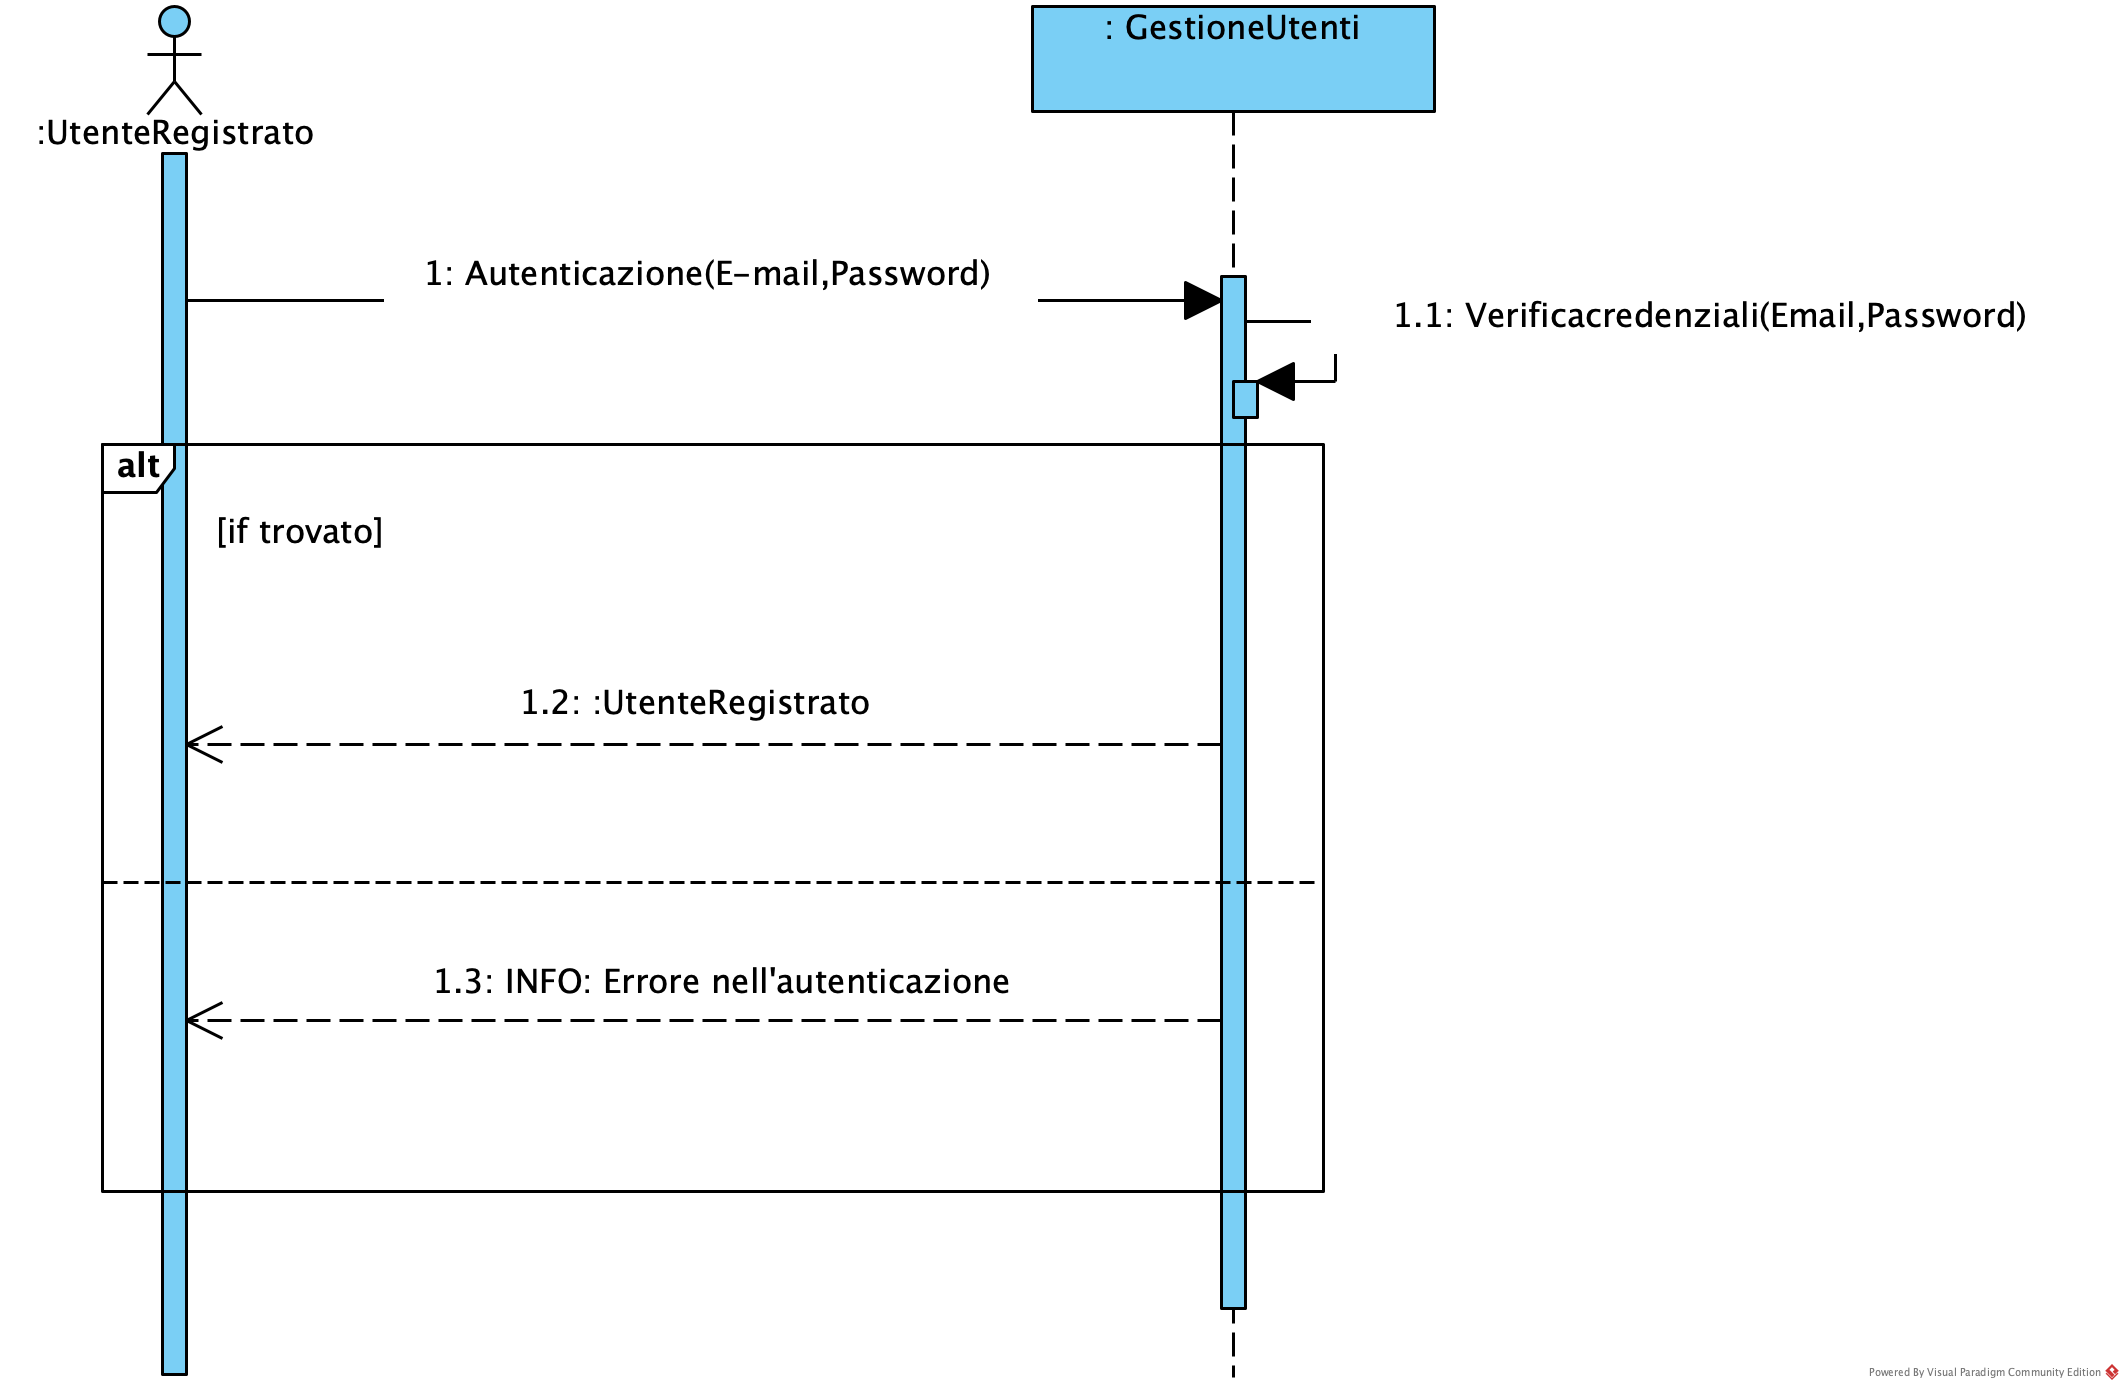
\includegraphics[width=0.8\linewidth]{assets/casid'uso/Autenticazione.png}
	\vspace{1ex}
    \textbf{Figura:} Diagramma di sequenza per il caso d’uso \textit{Autenticazione}
\end{figure}

\subsection{PubblicaEvento}

\begin{center}
    La creazione del seguente diagramma di sequenza, sviluppato a partire dalla descrizione dello scenario del caso \noindent d’uso \textit{PubblicaEvento}, ha fatto emergere la necessità di definire un metodo privato, specifico della classe \textbf{Amministratore}:

    \vspace{1ex}
    \textbf{verificaValidità(Titolo, Descrizione, Data, Orario, Luogo, NumMassimoPartecipanti)}
    
    \vspace{2ex}
    Tale metodo consente all’amministratore di verificare che i dati inseriti siano validi prima della pubblicazione di un evento.

    \vspace{3ex}
    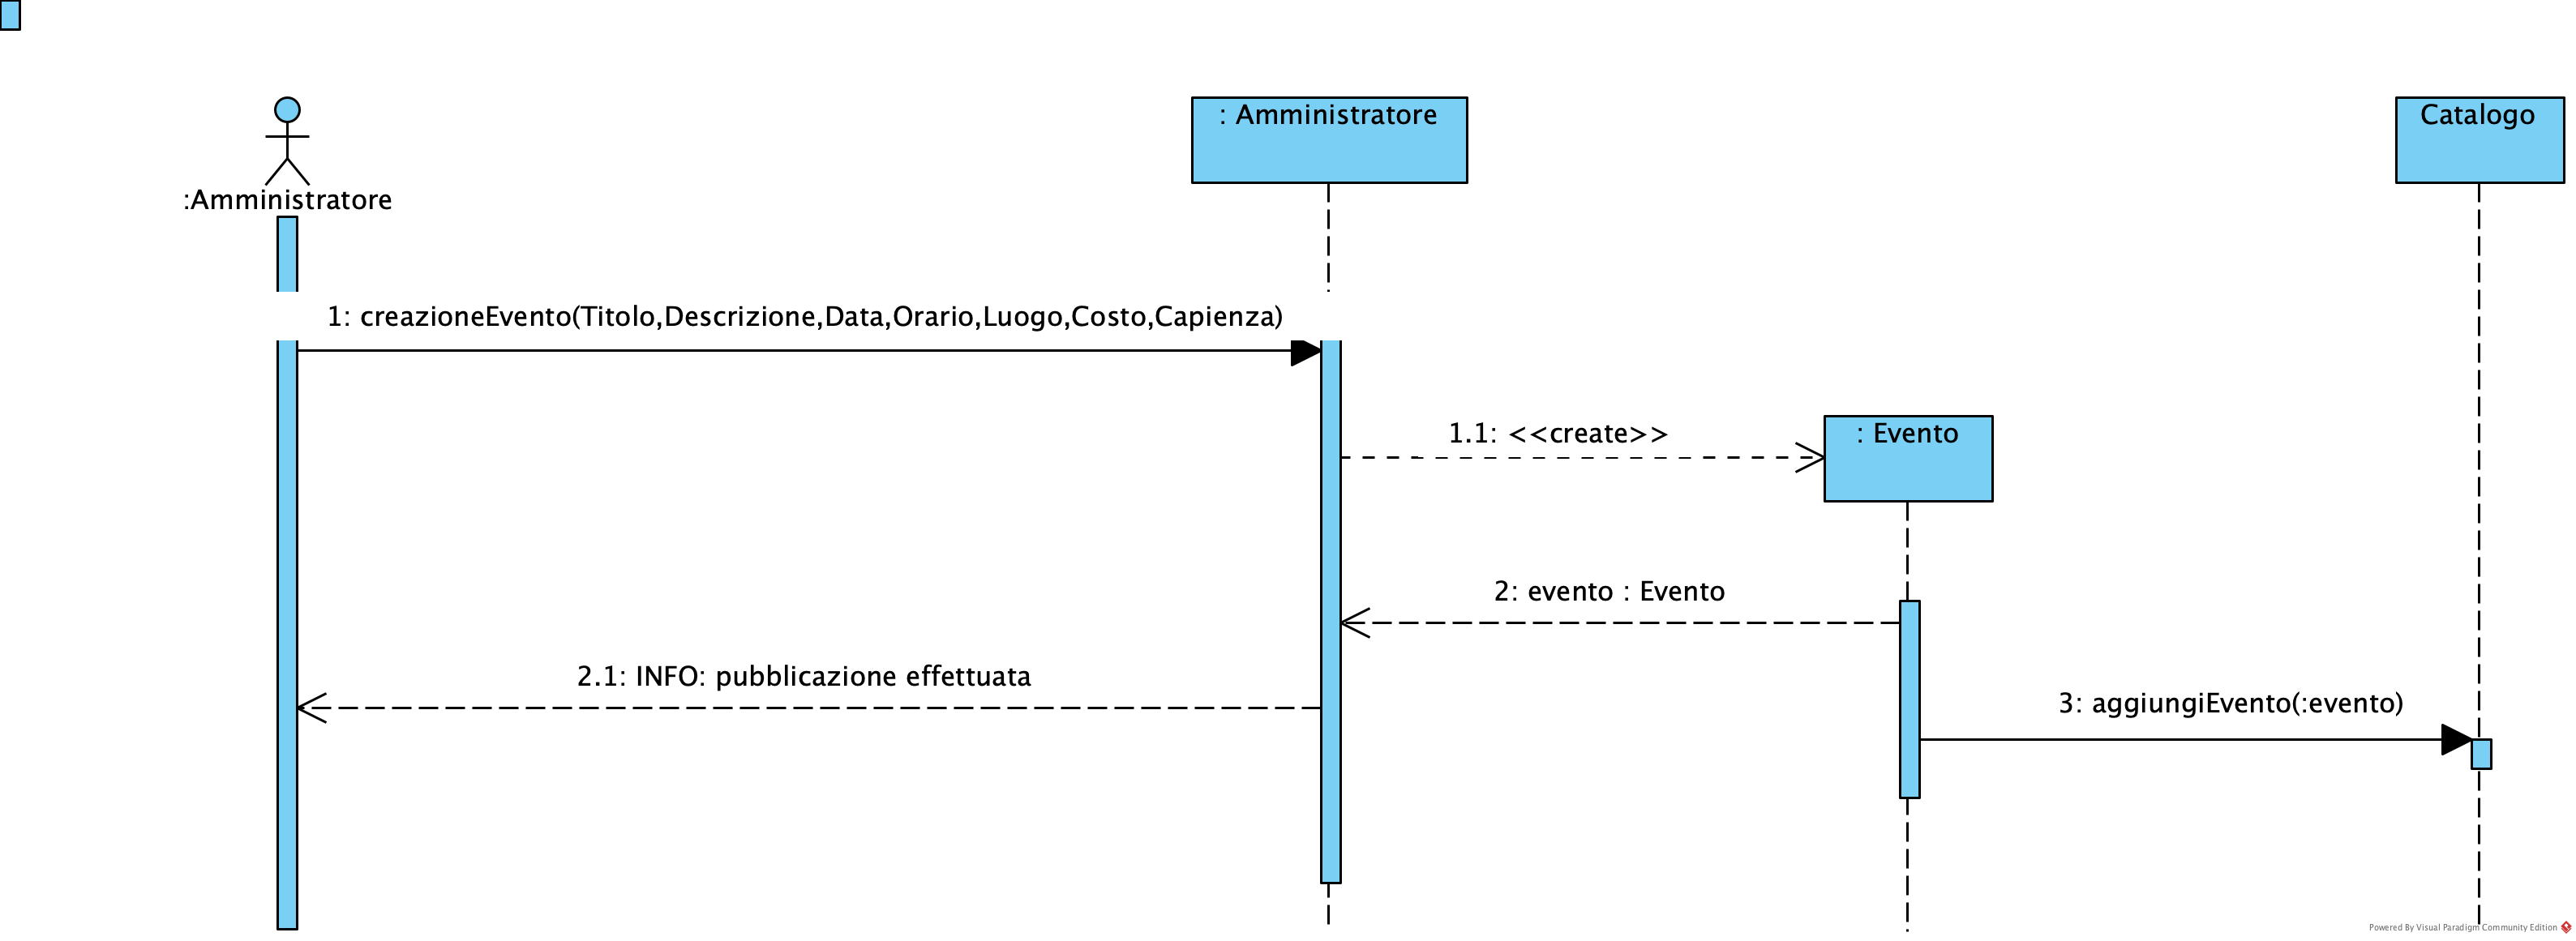
\includegraphics[width=\linewidth]{assets/casid'uso/PubblicaEvento.png}
    
    \vspace{1ex}
    \textbf{Figura:} Diagramma di sequenza per il caso d’uso \textit{PubblicaEvento}
\end{center}


\subsection{ConsultaEventiPubblicati}

\begin{center}
    Il diagramma di sequenza del caso d'uso \textit{ConsultaEventiPubblicati} mostra la necessità di una responsabilità \textbf{getListaPartecipanti()} da parte dell'evento

    \vspace{2ex}
    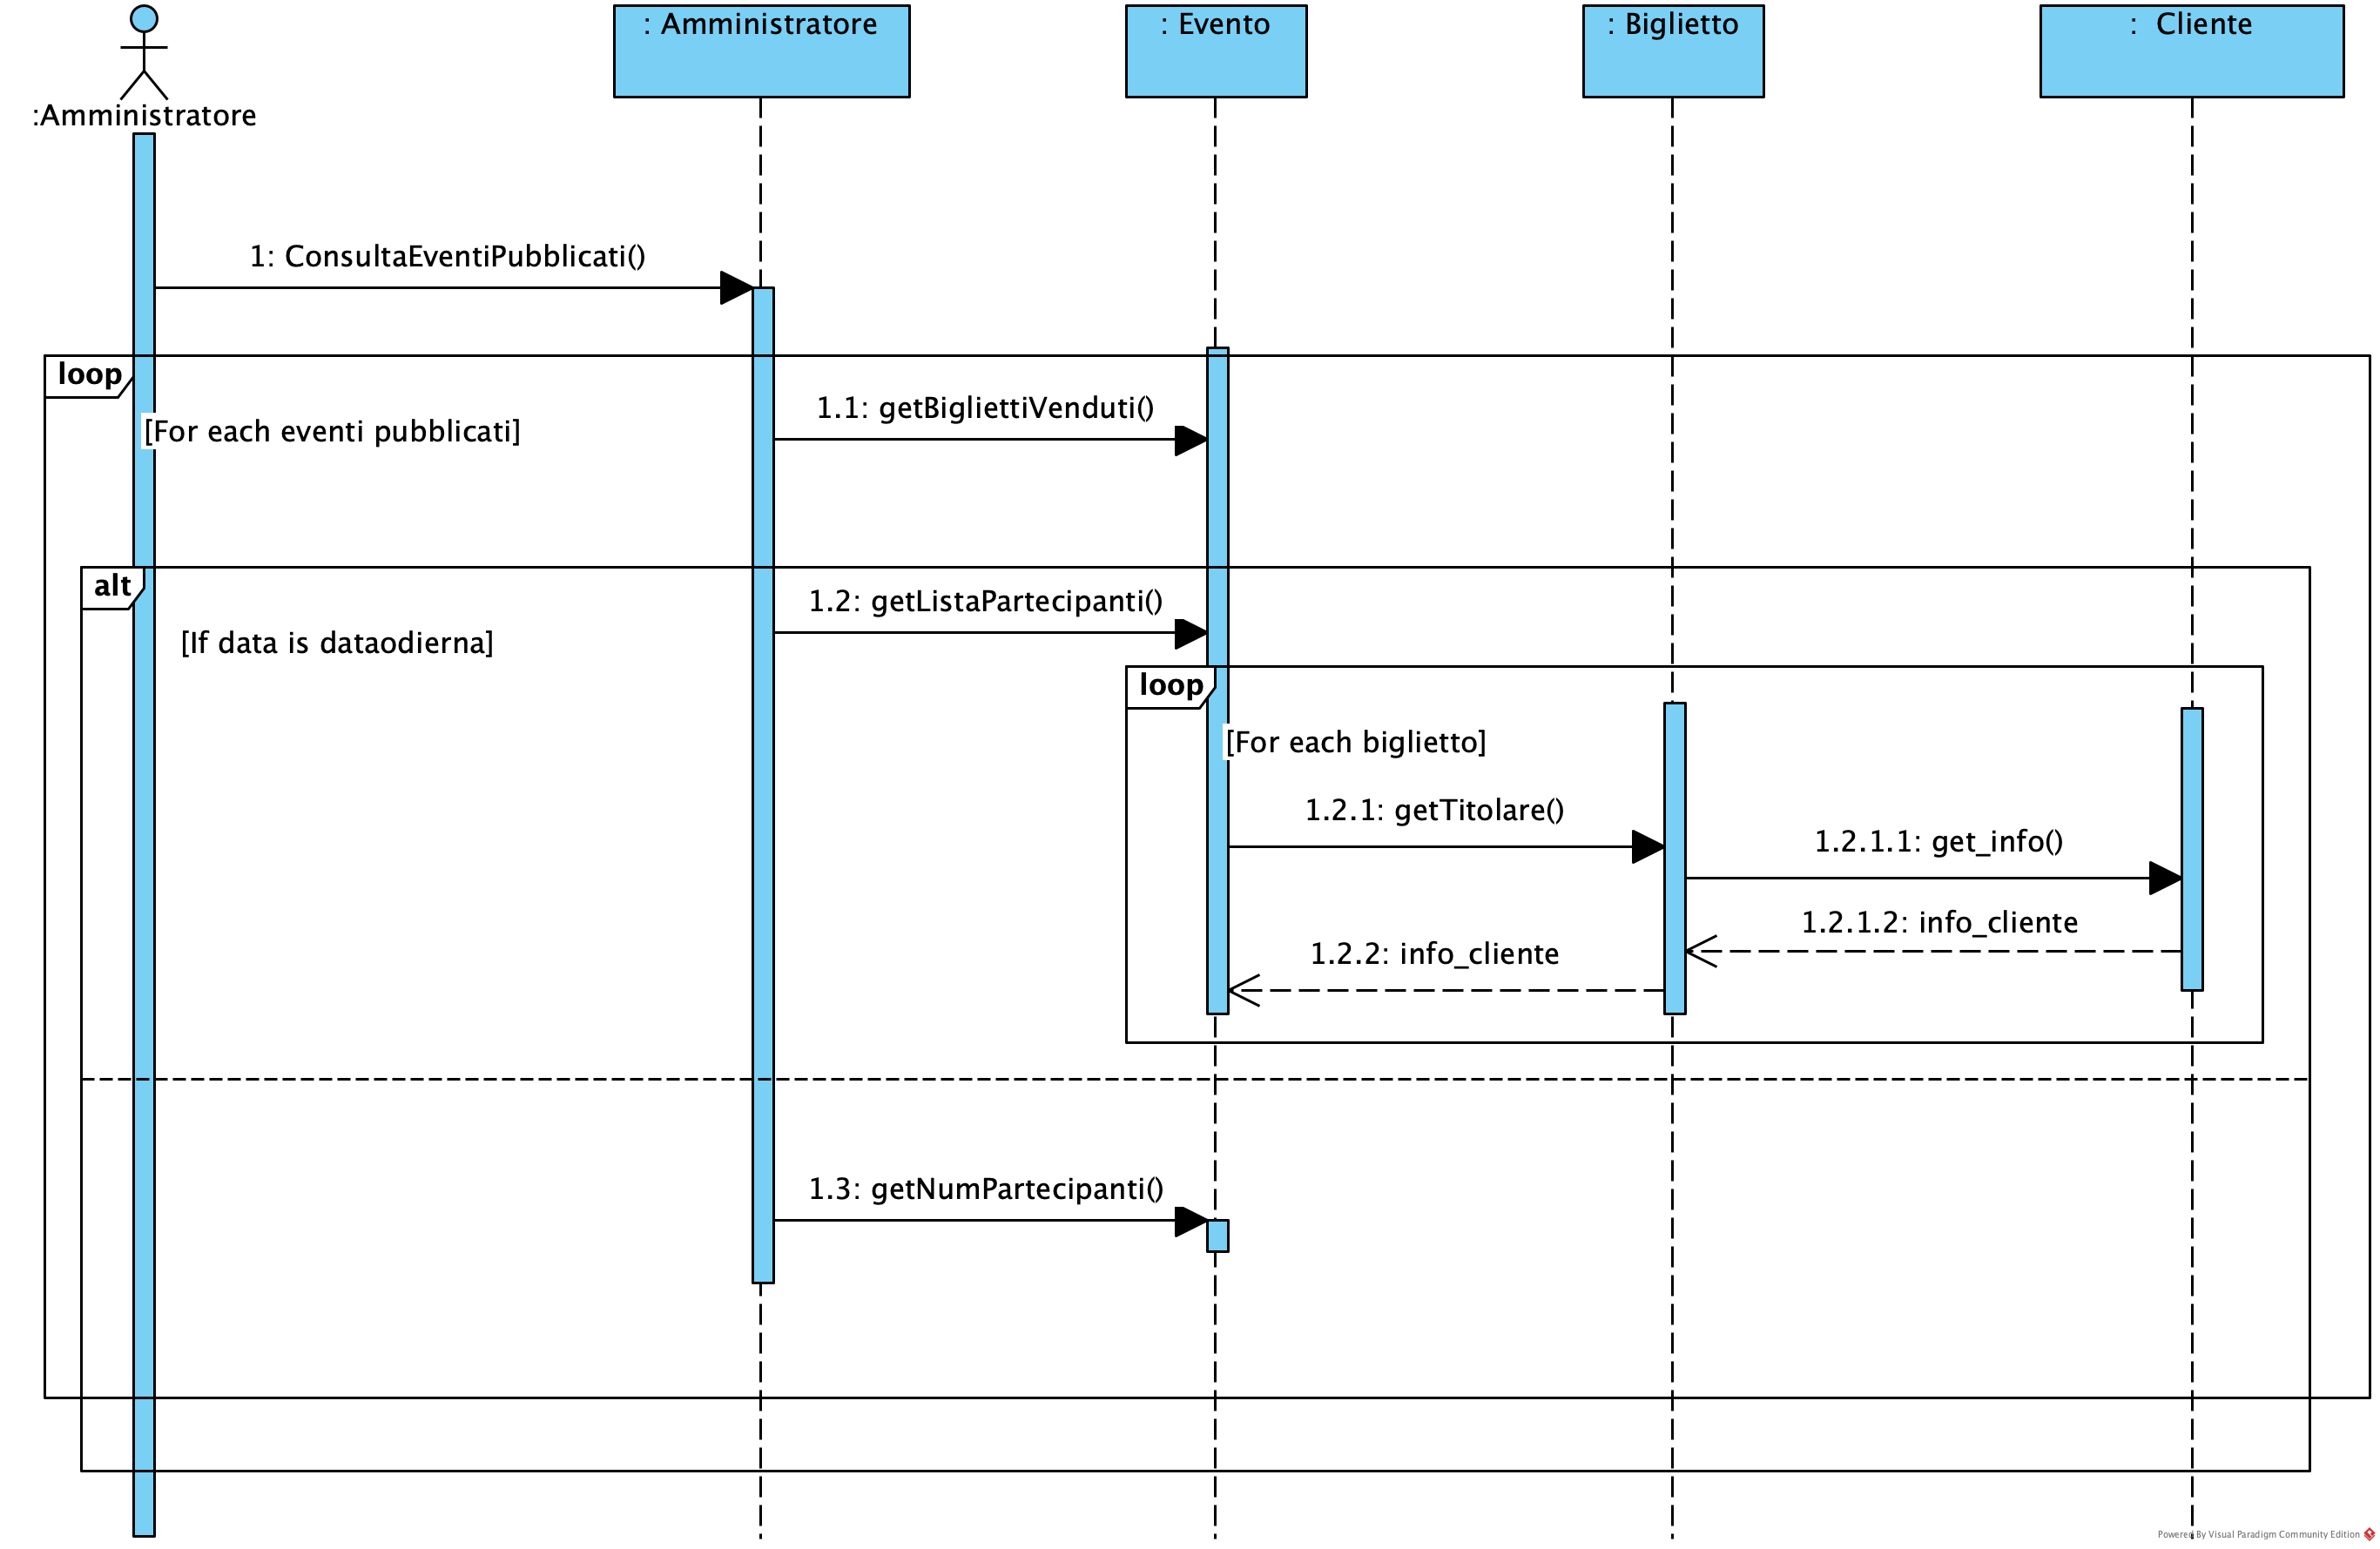
\includegraphics[width=0.8\linewidth]{assets/casid'uso/ConsultaEventiPubblicati.png}

    \vspace{1ex}
    \textbf{Figura:} Diagramma di sequenza per il caso d’uso \textit{ConsultaEventiPubblicati}
\end{center}


\newpage
{
\subsection{AcquistoBiglietti}

\begin{center}
Il diagramma di sequenza del caso d’uso \textit{AcquistoBiglietto} mostra il processo di acquisto da parte dell’utente. Durante questo flusso emergono tre nuove responsablità per la classe Evento: \textbf{verificaDisponibilità()}, \textbf{creazioneIdUnivoco()} e \textbf{InviaDatiPagamento(Nome, Cognome, Email, informazioniCarta)}. 
\vspace*{2mm}
\raisebox{2mm}{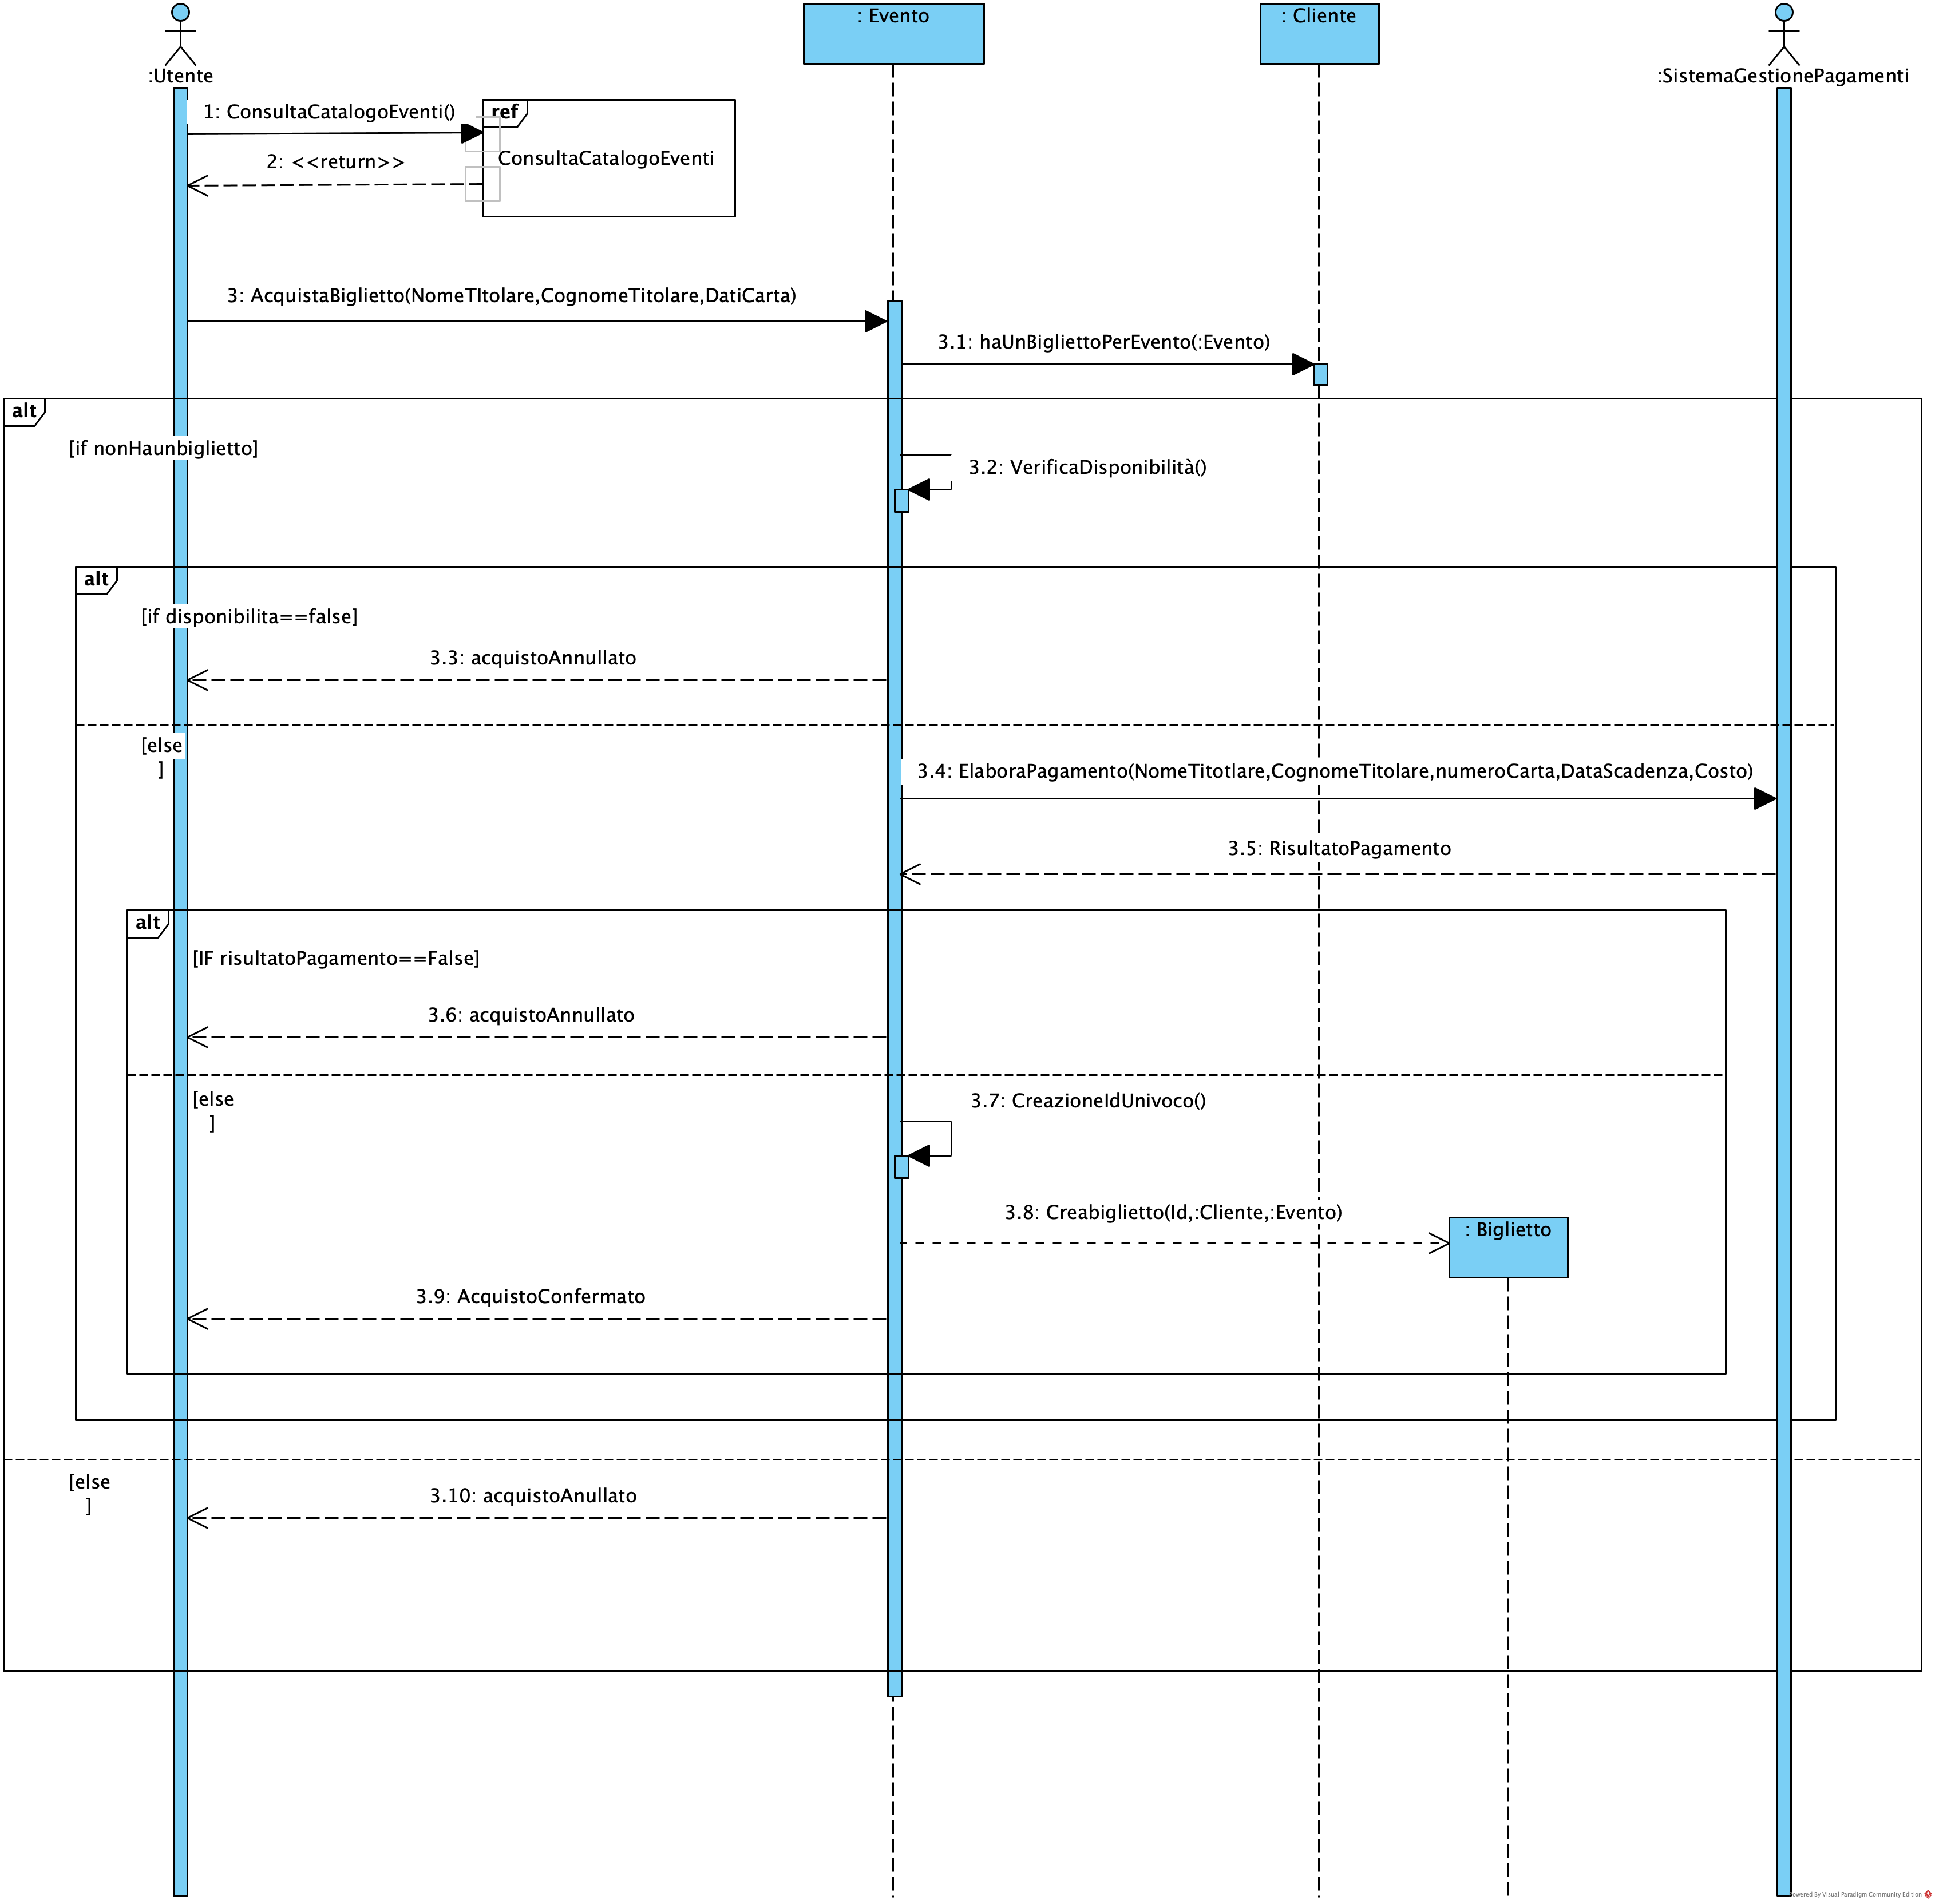
\includegraphics[width=0.8\linewidth]{assets/casid'uso/AcquistoBiglietto.png}}

\vspace{1ex}
\textbf{Figura:} Diagramma di sequenza per il caso d’uso \textit{AcquistoBiglietto}
\end{center}
}

\vspace{2ex}

{\small
\newpage
\subsection{PartecipazioneEvento}

\begin{center}
Il diagramma di sequenza del caso d’uso \textit{PartecipazioneEvento} evidenzia i passi necessari durante la partecipazione ad un evento da parte di un utente. E' stato necessario dunque aggiungere, come visibile dal diagramma, un nuovo metodo nella classe Evento: \textbf{verificaCodice()}, ed un nuovo metodo nella classe Biglietto: \textbf{validaBiglietto()}

\vspace{1ex}
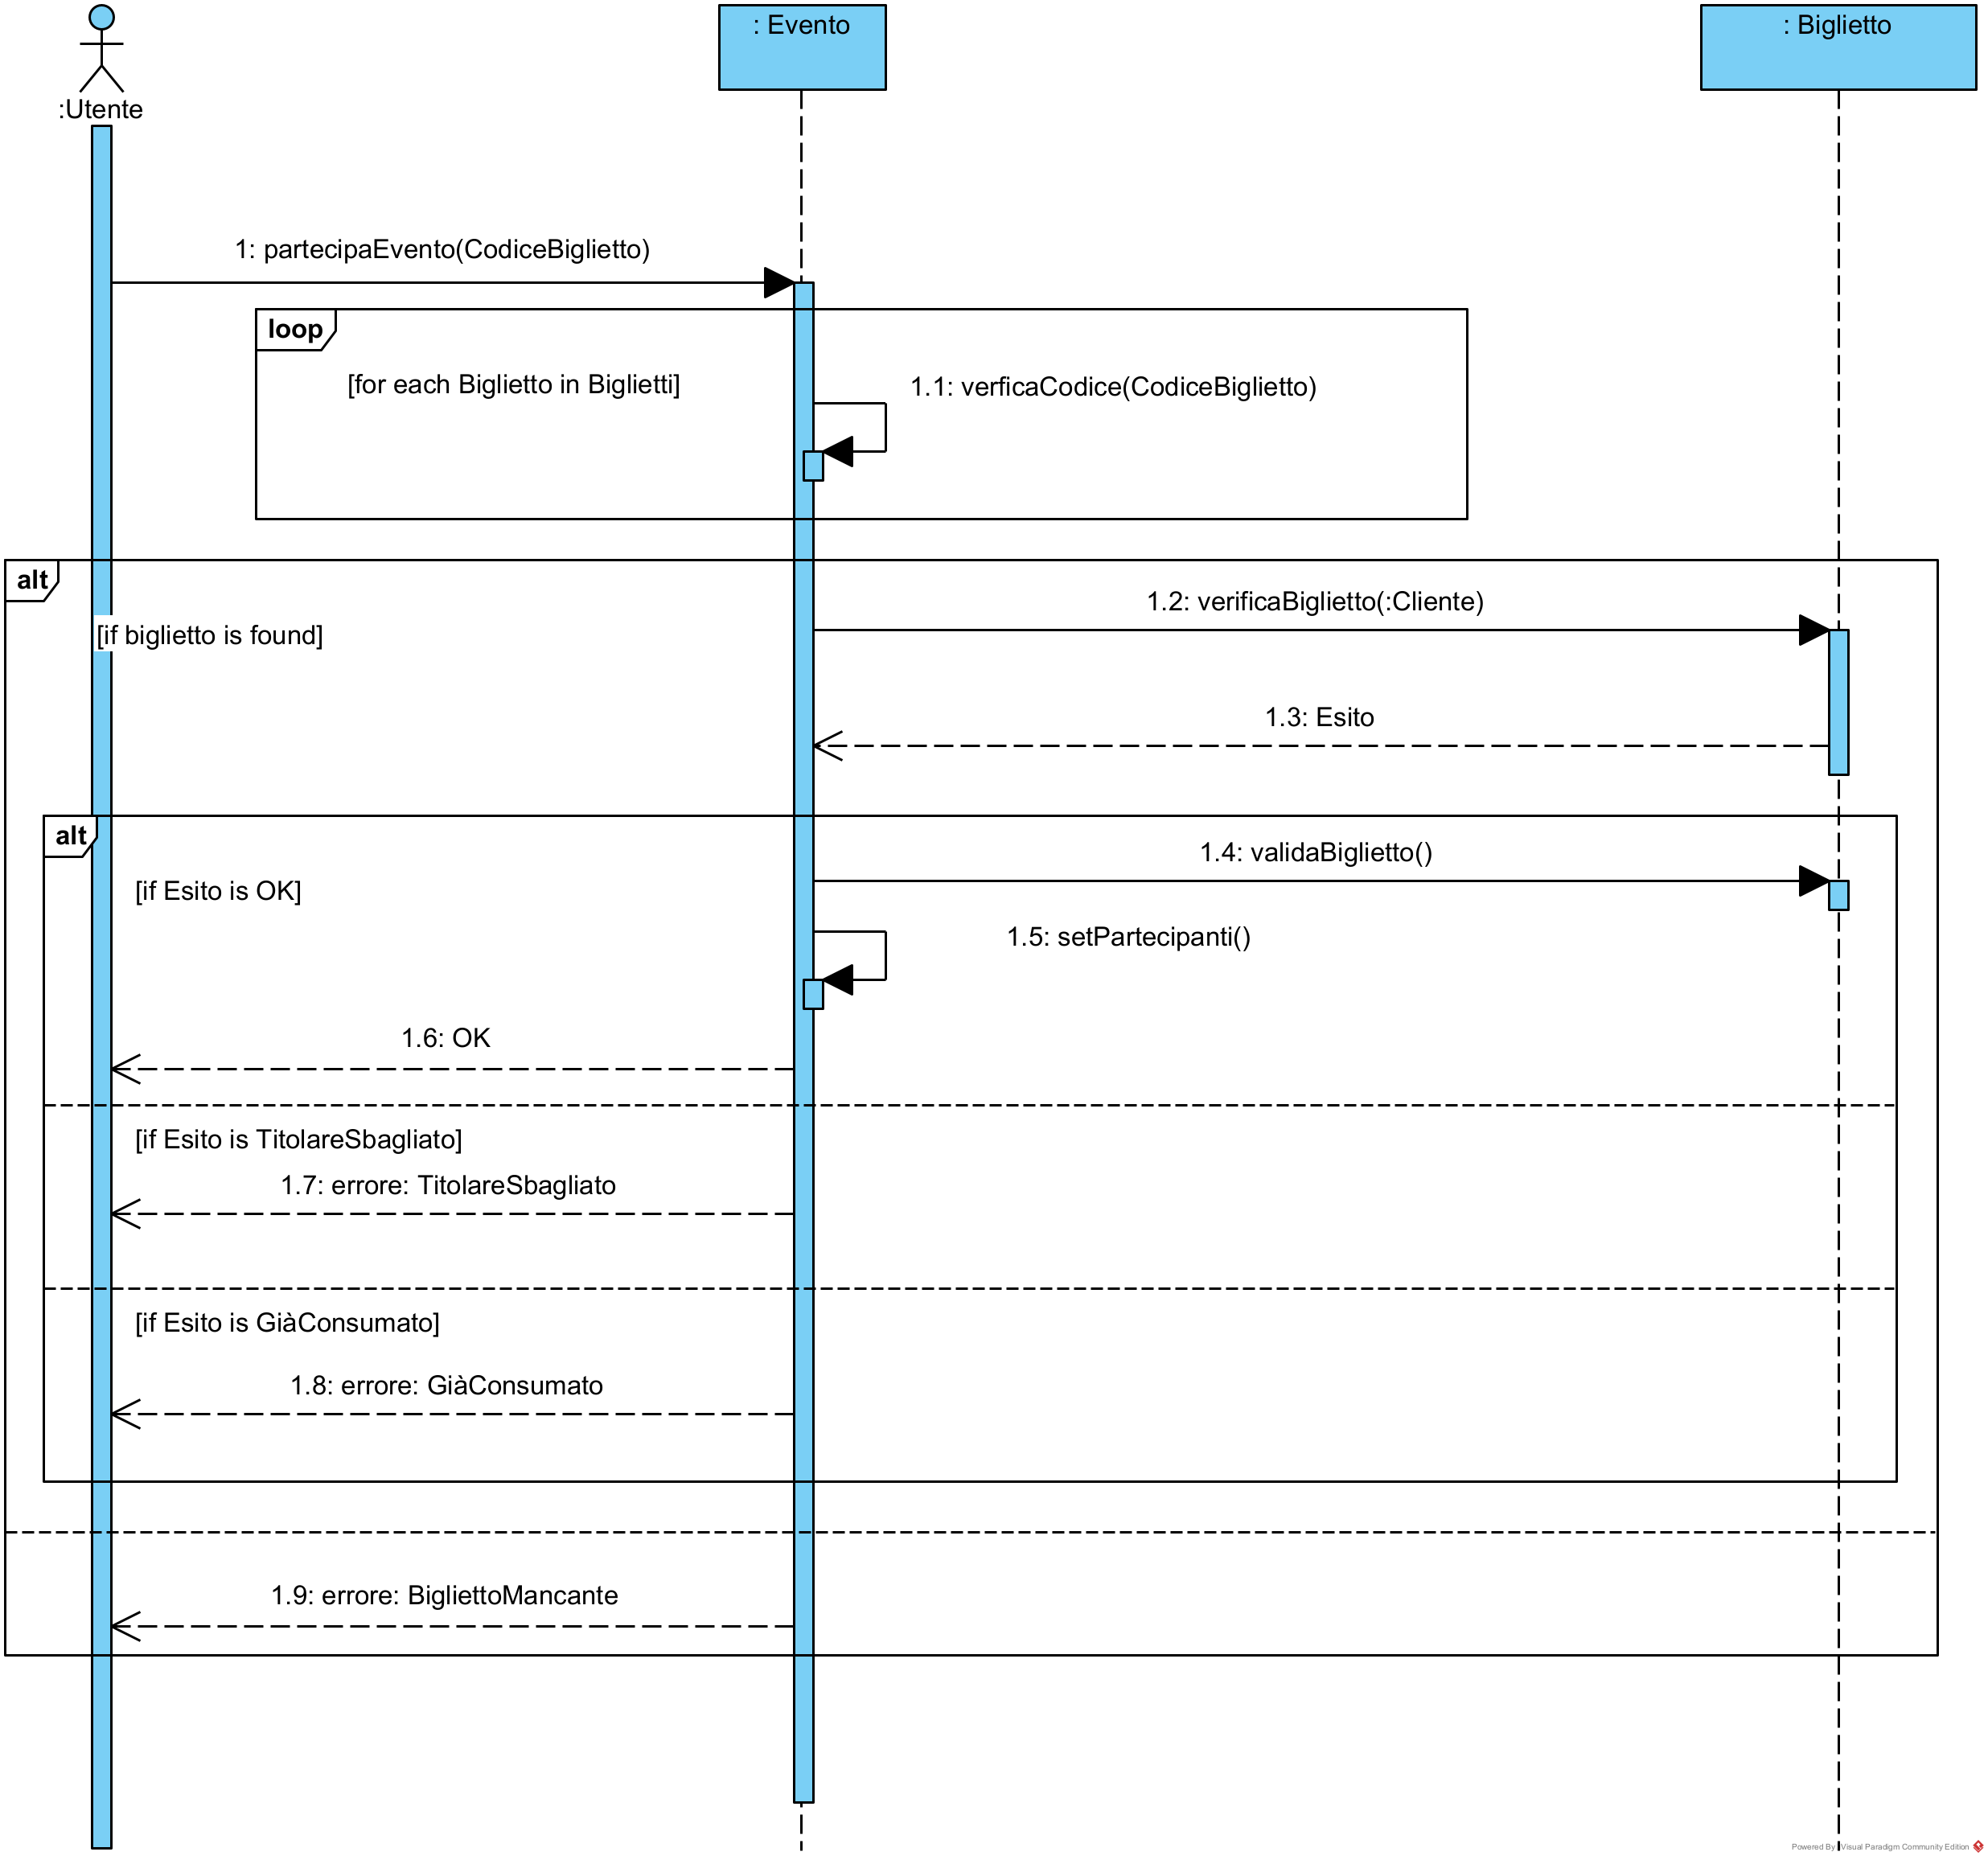
\includegraphics[height=0.38\textheight]{assets/casid'uso/PartecipazioneEvento.png}
\vspace{1ex}
\end{center}
\subsection{ModificaDatiPersonali}
\begin{center}
Come visibile dal sequence diagram del caso d'uso 
\textit{ModificaDatiPersonali} è stato necessario fornire alla classe \textbf{Cliente} un metodo privato, di istanza \textbf{VerificaDato(Dato,Valore)}

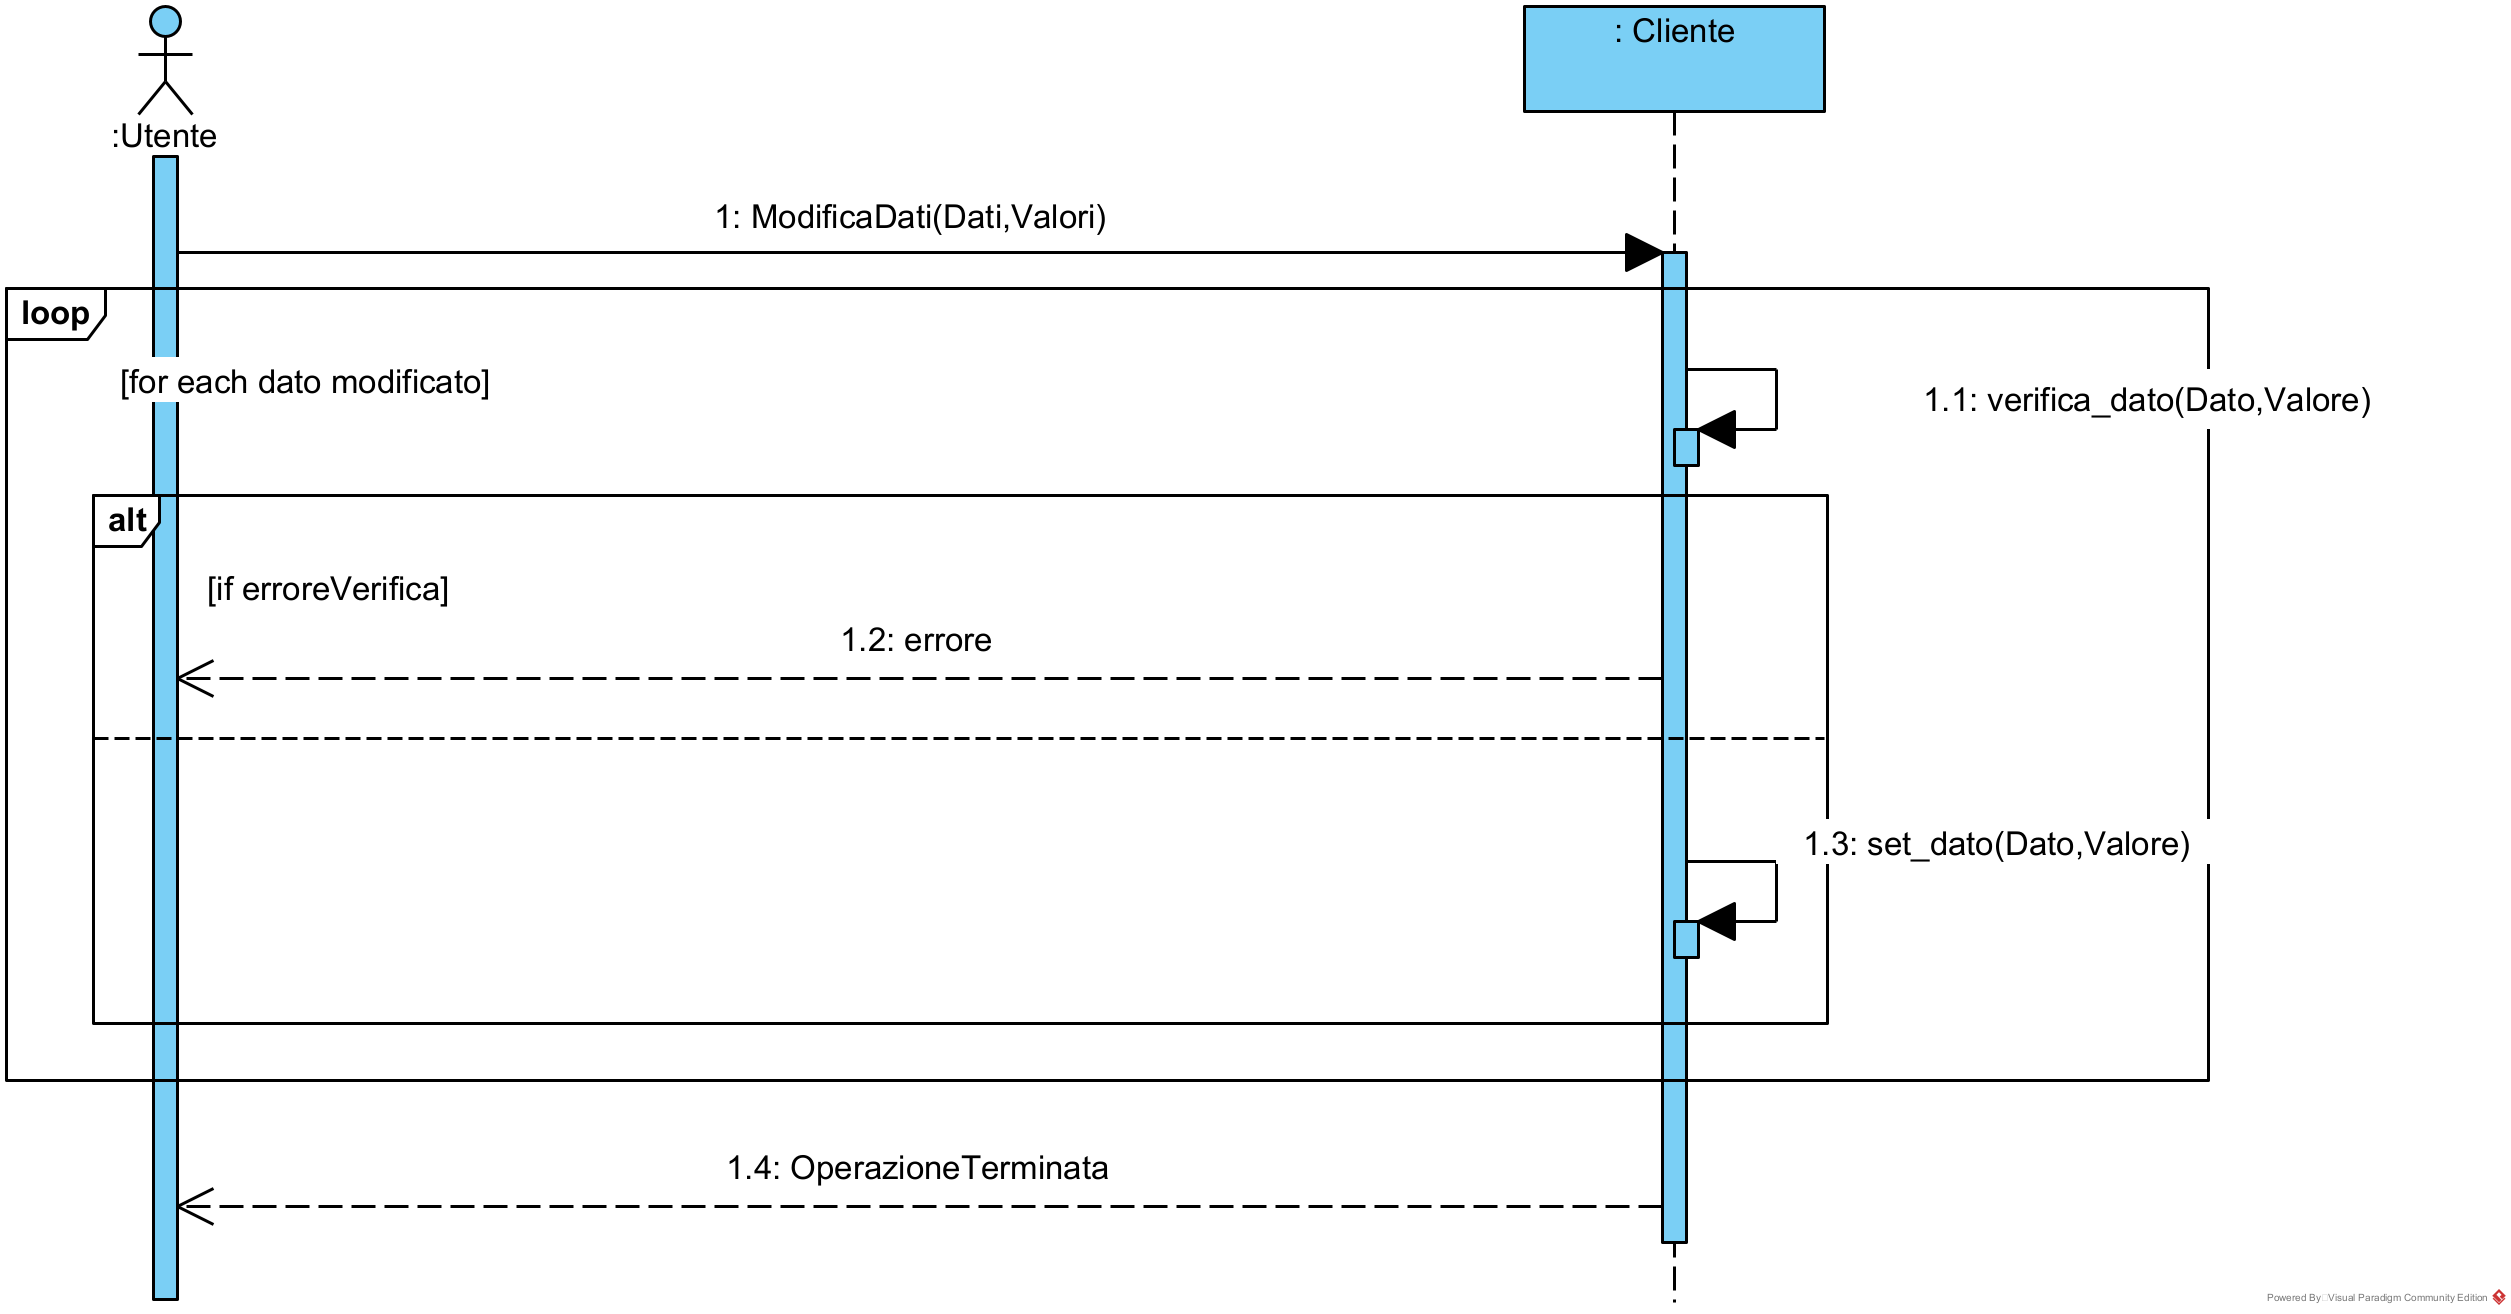
\includegraphics[height=0.38\textheight]{assets/casid'uso/ModificaDatiPersonali.png}
\vspace{1ex}
\end{center}

Il diagramma delle classi risultante è il seguente
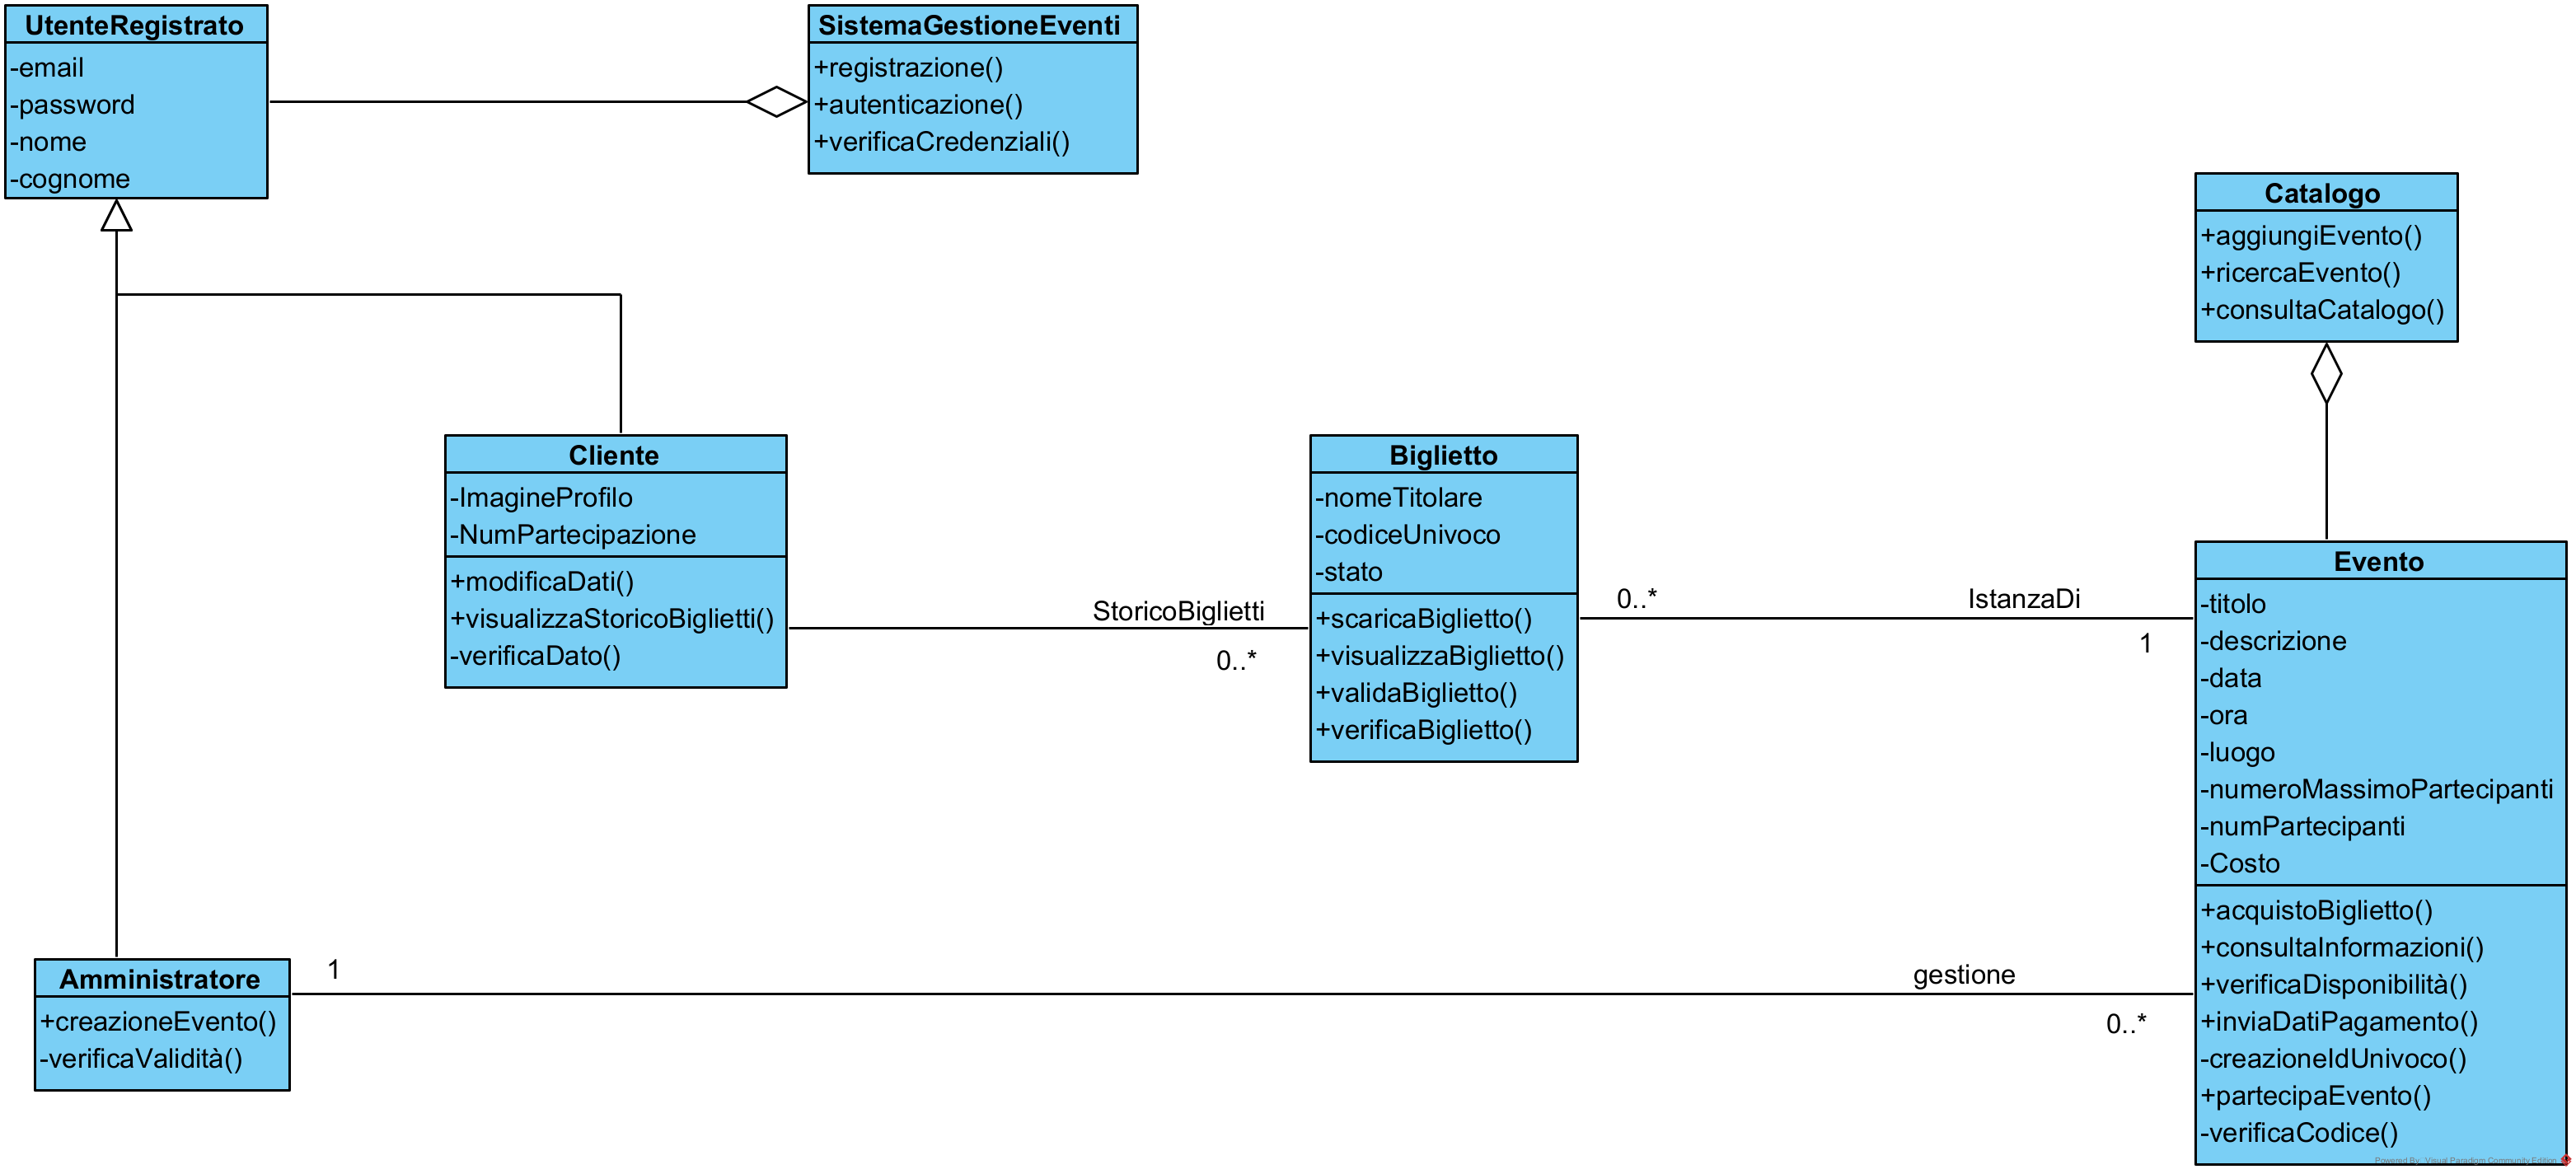
\includegraphics[height=0.38\textheight]{assets/casid'uso/DiagrammaClassiAggiornatoVero.png}
